
% % Uncomment to build this alone without subfiles:
% % (also stuff at bottom)
% \documentclass{scrbook}
% % \documentclass[draft]{scrbook}
% % Koma script document options
\KOMAoption{paper}{a4}
\KOMAoption{fontsize}{11pt}
\KOMAoption{parskip}{half-} % paragraph spacing
% \KOMAoption{numbers}{enddot} % dot after section number
\KOMAoption{cleardoublepage}{plain} % include page numbers on blank pages
\KOMAoption{chapterprefix}{true} % 'Chapter' before number

% Packages
\usepackage{amsmath} % Gives \text command inside maths blocks
\usepackage{amssymb} % Various maths symbols
\usepackage{array} % Table formatting
\usepackage{bm} % Bold maths including Greek
\usepackage[format=plain]{caption} % Font sizing and alignment in captions
\usepackage{enumitem} % Allows numbering like 1.1 in ordered lists
% \usepackage{float} % Allows H placement of floats
\usepackage{graphicx}
\usepackage[hidelinks]{hyperref} % Hyperlinks without looking like it
% \usepackage{longtable} % Multi-page tables
% \usepackage{multicol} % For columns in text (not tables)
\usepackage{multirow} % For tables
\usepackage{neuralnetwork} % Neural net diagram
\usepackage{pdflscape} % Gives landscape environment
% \usepackage{scrlayer-scrpage} % To move page numbers
\usepackage{tabularx}
\usepackage{textcomp} % Added to fix \textasciiacute error on laptop
% \usepackage{tikz} % Diagrams (used for neural network example)
% \usepackage[pagenumberwidth=3em]{tocbasic}
% \usepackage{tocstyle} % ToC styling
\usepackage{upgreek} % Non-italic greek letters
\usepackage{xpatch} % Biblatex customisation

\usepackage[a4paper, inner=40mm, outer=15mm, top=30mm, bottom=30mm,footskip=15mm, headsep=15mm]{geometry}
% \usepackage[a4paper, inner=40mm, outer=30mm, top=50mm, bottom=50mm,footskip=20mm, headsep=20mm]{geometry} % footskip is space between footer (i.e. page number) and bottom of text
% min allowed is inner 40 mm, others 15 mm

\pagestyle{plain} % no header for front matter, overridden at end of front matter

% Caption setup
% \tablecaptionabove
\captionsetup[table]{labelsep=space}
% \captionsetup[table]{labelsep=space, skip=50pt, position=top}
\captionsetup[figure]{labelsep=space} % labelsep prevents dot followed by colon in captions

% Line spacing
\usepackage{setspace}
% \setstretch{1.4} % strangely this is > \onehalfspacing but < \doublespacing
\onehalfspacing
% \doublespacing

\raggedbottom % prevent huge spaces between paragraphs

% % % % % % % % % % % % % % % % % % % % % % % % %
% Font setup
% \usepackage{mathpazo} % Covers maths mode too
\usepackage[sc]{mathpazo} % Covers maths mode too, sc enables small caps
% \usepackage{palatino}
\usepackage[T1]{fontenc} % 8-bit font encoding
\addtokomafont{disposition}{\rmfamily} % Use serif throughout
% % % % % % % % % % % % % % % % % % % % % % % % %

% % % % % % % % % % % % % % % % % % % % % % % % %
% Section formatting setup
% \RedeclareSectionCommand[beforeskip=0pt]{chapter}
\RedeclareSectionCommand[beforeskip=0pt, innerskip=0pt]{chapter}
\RedeclareSectionCommand[beforeskip=10pt]{subsubsection}
\RedeclareSectionCommand[afterskip=1pt]{subsubsection}
% \setcounter{secnumdepth}{\subsubsectionnumdepth} % number up to subsubsections

% No dot after chapter number (https://tex.stackexchange.com/a/484727)
\renewcommand*{\chapterformat}{%
  \mbox{\chapappifchapterprefix{\nobreakspace}\thechapter
  \IfUsePrefixLine{}{\enskip}}%
}

% In the running header, separate chapter number and name with em dash
\renewcommand*{\chaptermarkformat}{%
\chapapp~\thechapter~---~}

% Create subsubsubsection below subsubsection but above paragraph, following https://tex.stackexchange.com/a/356574

\DeclareNewSectionCommand[
  style=section,
  counterwithin=subsubsection,
  afterskip=1pt,
  beforeskip=10pt,
  % afterskip=1.5ex plus .2ex,
  % beforeskip=3.25ex plus 1ex minus .2ex,
  % afterindent=false,
  level=\paragraphnumdepth,
  tocindent=10em,
  tocnumwidth=5em
]{subsubsubsection}
\setcounter{secnumdepth}{\subsubsubsectionnumdepth}
% \setcounter{tocdepth}{\subparagraphtocdepth}
\setcounter{tocdepth}{\subsubsubsectionnumdepth}

\RedeclareSectionCommands[
  level=\numexpr\subsubsubsectionnumdepth+1\relax,
  toclevel=\numexpr\subsubsubsectiontocdepth+1\relax,
  increaselevel,
]{paragraph,subparagraph}
\RedeclareSectionCommand[
  counterwithin=subsubsubsection,
  tocindent=12em,
  tocnumwidth=6em,
  beforeskip=10pt,
  afterskip=1pt, % line break after paragraph title
]{paragraph}
\RedeclareSectionCommand[
  tocindent=14em,
  tocnumwidth=7em,
  beforeskip=0pt
]{subparagraph}
% % % % % % % % % % % % % % % % % % % % % % % % %

% Autoref capitalisation
\def\chapterautorefname{Chapter}
\def\sectionautorefname{Section}
\def\subsectionautorefname{Section}
\def\subsubsectionautorefname{Section}

% % % % % % % % % % % % % % % % % % % % % % % % %
% Bibliography setup
\usepackage[backend=biber,
    % style=authoryear,
    style=authoryear-comp, % Don't repeat same author(s) in multiple citations
    giveninits=true,
    useprefix=true, % 'van der' etc.
    url=false,
    doi=false,
    isbn=false,
    eprint=false,
    uniquename=false, % Don't add initials in citation to disambiguate between authors with the same surname
    uniquelist=false, % Don't disambiguate in citation between different 'et al.' teams
    maxbibnames=10,
    minbibnames=10,
    maxcitenames=3,%  # 2,
    natbib, % Gives citep and citet commands
    labelalpha=true, % Use an 'alpha' label for each bib entry
    maxalphanames=1, % Use first author as the alpha label
    sorting=anyvt, % Sort by alpha (first author) then year
    block=par, % New line between 'blocks' of the bib entry
    dashed=false, % Reprint author list for each publication in bibliography
    sortcites=false % Show citations in the order supplied
]{biblatex}

% Citation/reference parameters
\renewcommand*{\nameyeardelim}{\addspace} % Space between author and year rather than comma
\renewcommand*{\finalnamedelim}{\addspace\&\addspace} % Ampersand rather than 'and'
\xpatchbibmacro{name:andothers}{{\finalandcomma}}{\addspace}{}{} % Space before 'et al.' rather than comma

% Citation-specific parameters
\DeclareCiteCommand{\blindcite}{\unspace}{}{}{\mancite} % Easy manual citations

% Reference-specific parameters
\AtEveryBibitem{\clearfield{title}} % Suppress title
\AtEveryBibitem{\clearfield{month}} % Suppress month
\DeclareNameAlias{author}{family-given} % Surname first for not just the first author
\DeclareNameAlias{editor}{family-given} % Same for editors
\renewbibmacro{in:}{} % Remove 'In:'
\DeclareFieldFormat{journaltitle}{#1} % Journal title in normal font rather than italics
\renewbibmacro*{volume+number+eid}{\printfield{volume}\printfield{number}\setunit{\addcomma\space}\printfield{eid}} % No dot after issue
\DeclareFieldFormat[article]{number}{\mkbibparens{#1}} % Volume in brackets
\DefineBibliographyStrings{english}{page = {}, pages = {}} % Suppress 'p.'/'pp.'
\renewbibmacro*{date+extradate}{\printtext{\printfield{year}\addcomma}} % Year not in brackets
\DeclareFieldFormat{pages}{\mkfirstpage[{\mkpageprefix[bookpagination]}]{#1}} % Only give starting page
\DeclareFieldFormat{url}{\url{#1}} % No 'URL' before URLs
% \renewcommand{\finentrypunct}{} % Remove final full stop
\renewcommand*{\newunitpunct}{\addcomma\space} % Commas between elements of bibitems

\DeclareBibliographyDriver{book}{%
  \printnames{author}%
  \space
  \printfield{year}%
  \newunit\newblock
  \printfield{booktitle}%
  \newunit
  , \printlist{publisher}%
\finentry}

\DeclareBibliographyDriver{inproceedings}{%
  \printnames{author}%
  \space
  \printfield{year}%
  \newunit\newblock
  \printfield{booktitle}%
  \newunit
  \printfield{volume}%
  \newunit
  \printfield{pages}%
\finentry}

\DeclareBibliographyDriver{incollection}{%
  \printnames{author}%
  \space
  \printfield{year}%
  \newunit\newblock
  \printfield{booktitle}%
  \newunit
  , ed. \printnames{editor},%
  \newunit\newblock
  \printlist{publisher}%
\finentry}

\DeclareBibliographyDriver{misc}{%
  \printnames{author}%
  \space
  \printfield{year}%
  \newunit\newblock
  \printfield{title}%
  \newunit
  \printfield{url}%
\finentry}

\addbibresource{refs.bib}
% % % % % % % % % % % % % % % % % % % % % % % % %

% Footnote spacing
% \deffootnote[1em]{1.5em}{1em}{\textsuperscript{\thefootnotemark~}}
\deffootnote[1em]{1em}{1em}{\textsuperscript{\thefootnotemark~}}

% Testing setting all penalties to zero
\binoppenalty=0
\brokenpenalty=0
\clubpenalty=0
\displaywidowpenalty=0
\exhyphenpenalty=0
\floatingpenalty=0
\hyphenpenalty=0
\interlinepenalty=0
% \linepenalty=0 % allowing this to be zero splits titles in a strange way
\postdisplaypenalty=0
\predisplaypenalty=0
\relpenalty=0
\widowpenalty=0

% Shorthands (non-Maths)
\newcommand{\lcdm}{$\Lambda$CDM}
\newcommand{\wcdm}{$w$CDM}
\newcommand{\Euclid}{\textit{Euclid}}
\newcommand{\Planck}{\textit{Planck}}
\newcommand{\Pcl}{Pseudo-$C_\ell$}
\newcommand{\pcl}{pseudo-$C_\ell$}
\newcommand{\ttp}{3$\times$2\,pt}

% Maths shorthands
\newcommand{\alm}{a_{\ell m}}
\newcommand{\Cl}{C_\ell}
\newcommand{\fsky}{f_\text{sky}}
\newcommand{\lmax}{\ell_\text{max}}
\newcommand{\lmin}{\ell_\text{min}}
\newcommand{\leff}{\ell_\text{eff}}
\newcommand{\tmin}{\theta_\text{min}}
\newcommand{\mathbfit}[1]{\bm{\mathit{#1}}}
\newcommand{\mathbfss}[1]{\bm{\mathsf{#1}}} % to match MNRAS \mathbfss
\renewcommand{\Re}{\operatorname{Re}}
\renewcommand{\Im}{\operatorname{Im}}

% ΛCDM parameters (maths mode)
\newcommand{\wo}{w_0}
\newcommand{\wa}{w_a}
\newcommand{\omm}{\Omega_\text{m}}
\newcommand{\omb}{\Omega_\text{b}}
\newcommand{\omc}{\Omega_\text{c}}
\newcommand{\sie}{\sigma_8}

% % Editing only
% \usepackage{xcolor}
% \newcommand{\todo}[1]{\textbf{{\color{red}{#1}}}}


% \usepackage{subfiles} % Best to do this last apparently

% \pagestyle{headings}
% \setcounter{chapter}{0} % deliberately 1 too low
% \begin{document}

% Uncomment to use subfiles:
% \documentclass[../Thesis.tex]{subfiles}
% \begin{document}

\chapter{Cosmology}
\label{chap:cosmo}
\graphicspath{{../Figs/cosmo/}{Figs/cosmo/}}

Cosmology is the study of the Universe, the components that make it up, and its past and future evolution.

This chapter begins with an overview of the current standard model of cosmology in \autoref{co_Sec:std_model}, before outlining some of the key questions that remain unanswered in \autoref{co_Sec:open_questions}. A description of the main observational probes for learning about cosmology is given in \autoref{co_Sec:obs_probes}, before \autoref{co_Sec:weak_lensing} introduces the main such probe considered in this thesis: weak gravitational lensing.

\section{Standard cosmological model}
\label{co_Sec:std_model}

The concept of a standard model of cosmology refers to the simplest model that is consistent with all observational data to date.

The most minimal version of the standard cosmological model is called \lcdm{}, which stands for its two largest constituents: dark energy in the form of a cosmological constant ($\Lambda$) and cold dark matter (CDM). These will be described in more detail in \autoref{co_Sec:constituents}. This model has six free parameters, which are described in \autoref{co_Sec:free_params}, but is also extendable with additional parameters. For example, time-varying dark energy may be included using the dark energy equation of state parameter $w$ (see \autoref{co_Sec:dark_energy}), in which case the model is sometimes known as $w$CDM.

\subsection{Cosmological principle and anisotropies}

The most fundamental aspect of the standard cosmological model is the cosmological principle, which states that on sufficiently large scales, the Universe is homogeneous and isotropic, meaning that it is the same everywhere and in all directions.

However, the Universe is not completely isotropic. This is self-evident on smaller scales, where we observe structure such as planets, stars and galaxies. It is also the case on larger scales, where matter is distributed in the walls, filaments and voids that make up the `cosmic web', as seen in \autoref{co_Fig:cosmic_web}.

\begin{figure}
\centering
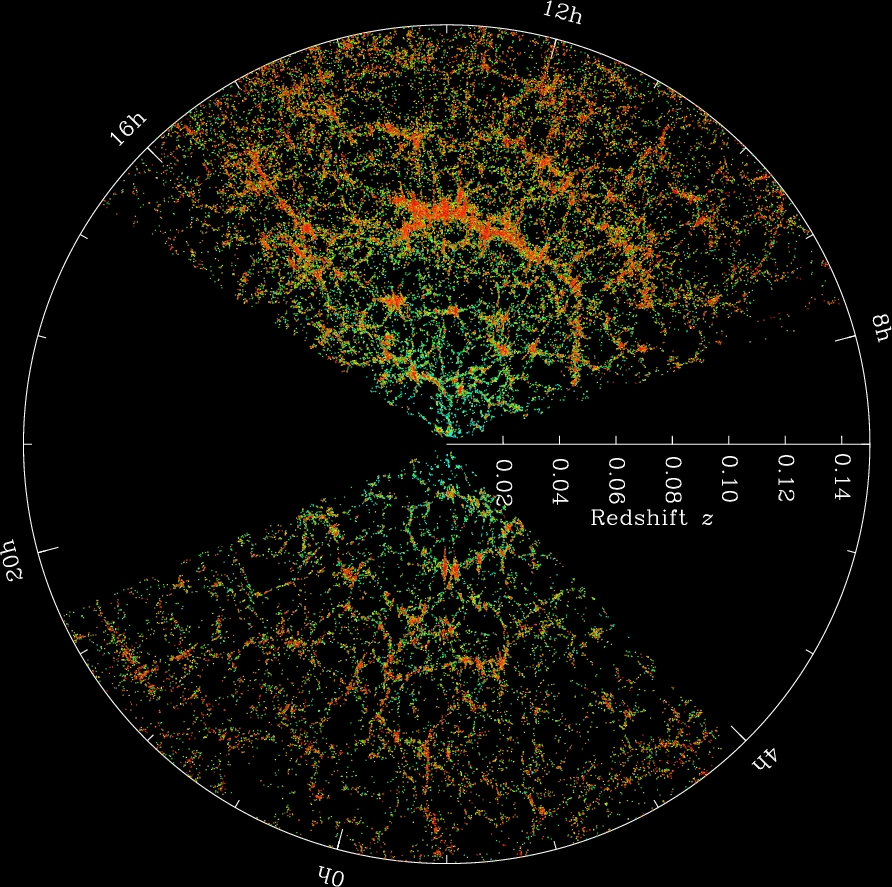
\includegraphics[width=\textwidth]{sdss}
\caption{The cosmic web of the large-scale matter distribution, as traced by galaxies detected by the Sloan Digital Sky Survey (SDSS; \cite{York2000}; \cite{Blanton2017}). Image by M. Blanton and SDSS.}
\label{co_Fig:cosmic_web}
\end{figure}

These anisotropies are believed to arise from quantum fluctuations in the early Universe, which later resulted in over- and underdense regions of matter, which evolved under gravity to give the structures we observe today. This is strongly supported by measurements of baryon acoustic oscillations (which will be described in \autoref{co_Sec:BAO}) and by observations of the cosmic microwave background (CMB), which have revealed that the early Universe was extremely smooth, with small anisotropies of order one part in $10^5$. The CMB and its anisotropies will be described in more detail in \autoref{co_Sec:CMB}.

\subsection{Cosmic expansion and redshift}

After the cosmological principle, perhaps the most fundamental aspect of the standard model of the Universe is that it is expanding. Mathematically, this can be described simply using the scale factor, $a \left( t \right)$, where any distance $d$ at time $t$ is given by
\begin{equation}
d \left( t \right) = a \left( t \right) d_0,
\end{equation}
where $d_0$ is the distance today ($t = t_0$), and the current value of the scale factor, $a_0$, is defined as
\begin{equation}
a_0 = 1.
\end{equation}

For any time in the past, $t < t_0$,
\begin{equation}
a \left( t < t_0 \right) < 1,
\end{equation}
and therefore distances were shorter than they are today. Rewound far enough, this implies that at one stage the Universe was infinitely dense. This is called the Big Bang, and is a central part of the standard cosmological model.

% If distances were shorter in the past, then so too were wavelengths of light and other radiation that was emitted at the time, and has been effectively stretched on its way to the observer.
If distances were shorter in the past, then so too were wavelengths of light and other radiation. The wavelength of any photon has subsequently been stretched between its emission in the past and its observation today.
This effect is called redshift. Since the finite speed of light means that observations of any distant object are equivalent to looking back in time, redshift is a useful measure of the distance of objects from the Earth. Redshift, $z$, can be quantified as
\begin{equation}
1 + z = \frac{\lambda_\text{obs}}{\lambda_\text{emit}}
= \frac{1}{a \left( t \right)},
\end{equation}
where $\lambda_\text{emit}$ and $\lambda_\text{obs}$ are the emitted and observed wavelengths of light.

Evidence for the expanding Universe comes from the Hubble law \citep{Lemaitre1927, Hubble1929}, which states that distant galaxies are receding at a speed $v$ proportional to their distance $d$:
\begin{equation}
v = H_0 d,
\label{co_Eqn:hubble_law}
\end{equation}
where the constant of proportionality is the Hubble constant $H_0$. Despite its name, $H_0$ is today considered as the current value of a time-varying parameter $H \left( t \right)$, which is related to the scale factor $a$ as
\begin{equation}
H = \frac{\dot{a}}{a},
\label{co_Eq:hubble_param}
\end{equation}
where the overdot denotes a time derivative. A more recent diagram of the Hubble law is shown in \autoref{co_Fig:hubble_diagram}. This was compiled from Type Ia supernovae, which will be described in \autoref{co_Sec:supernovae}, and is taken from \citet{Kirshner2004}. Strong evidence for the implied Big Bang is supplied by observations of the CMB (\autoref{co_Sec:CMB}).

\begin{figure}
\centering
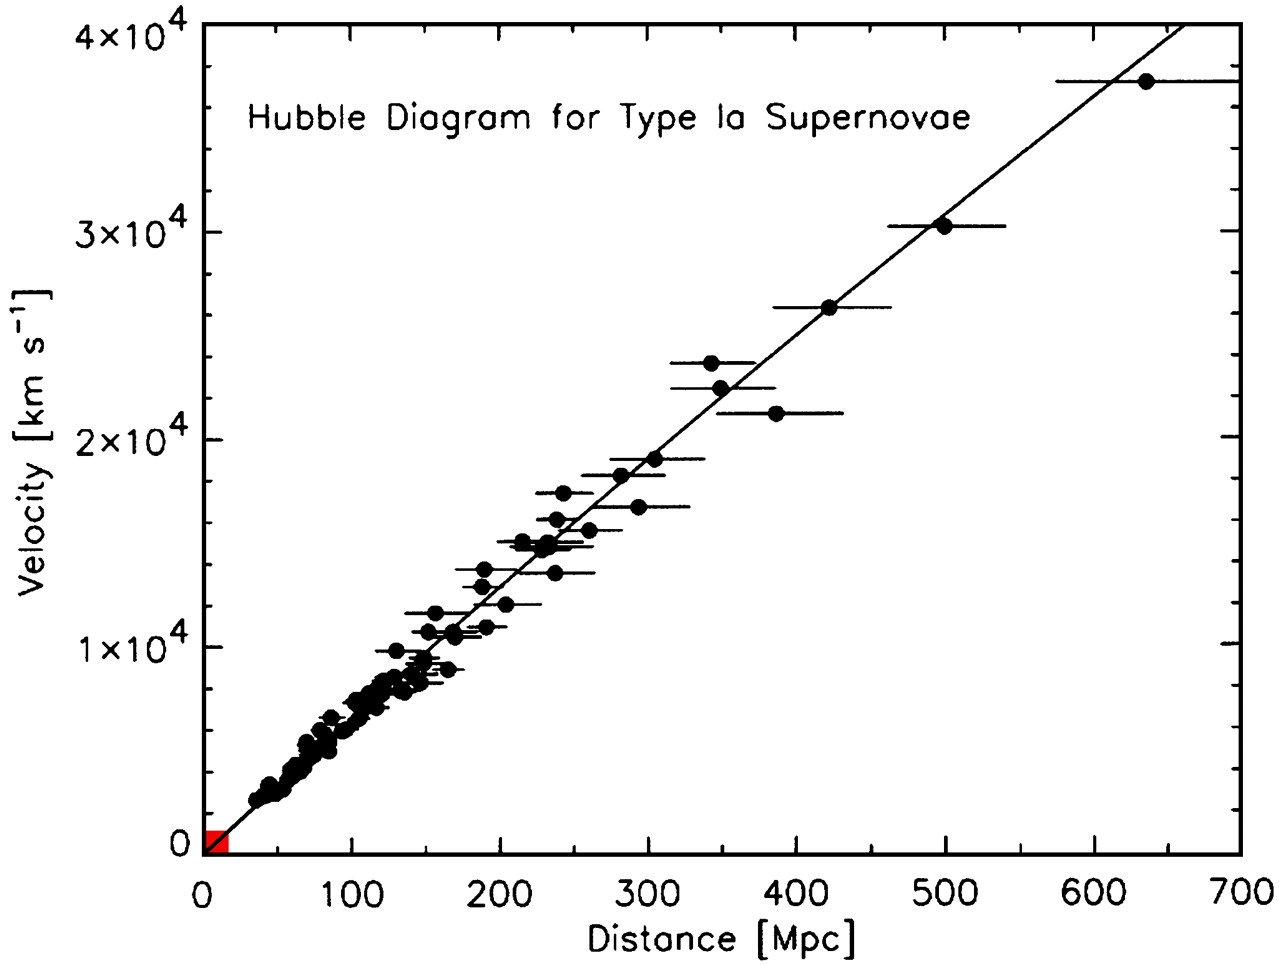
\includegraphics[width=.8\textwidth]{hubble_diagram}
\caption{Diagram of the Hubble law (\autoref{co_Eqn:hubble_law}) relating the recession velocity of distant objects (in this case Type Ia supernovae, which are described in \autoref{co_Sec:supernovae}) to their distance. Taken from \citet{Kirshner2004}.}
\label{co_Fig:hubble_diagram}
\end{figure}

\subsection{The FLRW Universe}

This section provides an overview of some of the mathematics underpinning the standard model of cosmology. It is named after four of its key contributors: Friedmann, Lema\^itre, Robertson and Walker.

In \lcdm{} and simple extensions such as $w$CDM, the Universe is governed by the theory of general relativity (GR), which describes the relationship between the geometry of the Universe and its contents. GR provides a near-universal theory of gravity covering both everyday and cosmological scales (though it notably fails on quantum scales). GR is summarised in the Einstein field equations, which may in fact be written as a single equation \citep{Einstein1916},
\begin{equation}
G_{\mu \nu} + \Lambda g_{\mu \nu}
= \frac{8 \pi G}{c^4} T_{\mu \nu}.
\label{co_Eqn:einstein}
\end{equation}
$G_{\mu \nu}$ in Equation \eqref{co_Eqn:einstein} is the Einstein tensor describing the curvature of spacetime, and $T_{\mu \nu}$ is the energy--momentum tensor describing the energy density at a given point in spacetime. $g_{\mu \nu}$ is the metric tensor, which describes the geometric and causal structure of spacetime, and is related to the separation between points in spacetime, which is discussed below. In Equation \eqref{co_Eqn:einstein} it multiplies the cosmological constant $\Lambda$, which could alternatively be absorbed into $T_{\mu \nu}$, where it could also be replaced with a time-varying dark energy contribution to the density. The Einstein field equations are related to the Newtonian theory of gravity through the classical gravitational constant $G$.

Distances between points in a homogeneous, isotropic and expanding Universe can be quantified using the FLRW metric, which decomposes the line element of spacetime $\text{d}s$ into contributions from time $\text{d}t$ and space, $\text{d}\Sigma$,
\begin{equation}
\text{d}s^2 = - c^2 \text{d}t^2 + a \left( t \right)^2
\text{d}\Sigma^2.
\end{equation}
The spatial metric is further decomposed, in hyperspherical coordinates, into a radial contribution $\text{d}\chi$ and an angular contribution $\text{d}\Omega$ as
\begin{equation}
\text{d}\Sigma^2 = \text{d}\chi^2 + S_K \left( \chi \right)^2
\text{d}\Omega^2.
\label{co_Eqn:spatial_metric}
\end{equation}
$\chi$ is the comoving angular distance, defined in terms of the scale factor $a$ as
\begin{equation}
\chi \left( a \right) = c \int_a^1 {
\frac{ \text{d}a' }{a'^2 H \left( a' \right)}
}.
\end{equation}
The angular line element $\text{d}\Omega$ is given in terms of polar and azimuthal contributions $\text{d}\theta$ and $\text{d}\phi$ as
\begin{equation}
\text{d}\Omega^2 = \text{d}\theta^2
+ \sin^2 \left( \theta \right) \text{d}\phi^2.
\end{equation}
$S_K \left( \chi \right)$ in Equation \eqref{co_Eqn:spatial_metric} is the comoving angular diameter distance, whose value depends on the curvature of the Universe $K$. Specifically, it takes different forms in three cases: a closed Universe with spherical geometry ($K > 0$), a flat Universe with Euclidean geometry ($K = 0$), or an open Universe with hyperbolic geometry ($K < 0$). The comoving angular diameter distance in each of these cases is given by
\begin{equation}
S_K \left( \chi \right) =
\begin{cases}
K^{-\frac{1}{2}} \sin{\left( K^{\frac{1}{2}} \chi \right)}
& \quad \text{for $K > 0$ (closed);} \\
\chi
& \quad \text{for $K = 0$ (flat);} \\
\left| K \right|^{-\frac{1}{2}}
\sinh{\left( \left| K \right|^{\frac{1}{2}} \chi \right)}
& \quad \text{for $K < 0$ (open).} \\
\end{cases}
\label{co_Eqn:angular_diameter_distance}
\end{equation}

The spacetime line element in the FLRW metric, $\text{d}s$, can be related to the metric tensor $g_{\mu \nu}$ from Equation \eqref{co_Eqn:einstein} as
\begin{equation}
\text{d}s^2 = g_{\mu \nu} \text{d}x^\mu \text{d}x^\nu,
\end{equation}
where $\text{d}x^\mu$ is the infinitesimal displacement in comoving coordinates; that is, spacetime coordinates defined such that the spatial component remains constant in the expanding Universe.

It is typical to model the constituents of the Universe as perfect fluids, which are completely described by their energy density $\rho$ and isotropic pressure $P$. Under this assumption, a solution to the Einstein field equations for a homogeneous, isotropic and expanding Universe governed by the FLRW metric is given by the Friedmann equations \citep{Friedmann1922, Friedmann1924},
\begin{equation}
H^2 = \left( \frac{\dot{a}}{a} \right)^2
= \frac{8 \pi G}{3} \rho
+ \frac{\Lambda c^2}{3}
- \frac{K c^2}{a^2};
\label{co_Eq:friedmann}
\end{equation}
\begin{equation}
\frac{\ddot{a}}{a} = - \frac{4 \pi G}{3}
\left( \rho + \frac{3 P}{c^2} \right) + \frac{\Lambda c^2}{3}.
\end{equation}

These two equations can be used to derive a third, the energy conservation equation:
\begin{equation}
\dot{\rho} = - 3 H \left( \rho + \frac{P}{c^2} \right).
\label{co_Eq:energy_conservation}
\end{equation}

Under the assumption that the constituents of the Universe may be modelled as perfect fluids, the equation of state relating the density $\rho_X$ and pressure $P_X$ for a given constituent $X$ is
\begin{equation}
P_X = w_X \rho_X c^2,
\end{equation}
where $w_X$ is the dimensionless equation of state parameter. In this thesis, the symbol $w$ will be used without any subscript to denote the equation of state parameter for dark energy. This parameter is discussed further in \autoref{co_Sec:dark_energy}.

The energy conservation equation (\autoref{co_Eq:energy_conservation}) may be used to derive an expression for the evolution of the density of constituent $X$:
\begin{equation}
\frac{\text{d} \ln{\rho_X}}{\text{d} \ln{a}} + 3 \left( 1 + w_X \right) = 0.
\end{equation}
When $w_X$ is constant, this equation has a solution,
\begin{equation}
\rho_X \propto a^{-3 \left( 1 + w_X \right)}.
\label{co_Eq:rho_dependence_on_a}
\end{equation}

When a given component is dominant, the resulting evolution of the scale factor as a function of time may be found by substituting $\rho_X$ into Equation \eqref{co_Eq:friedmann}. Values of $w_X$ for the different constituents of the Universe and the resulting evolution of the scale factor will be discussed in \autoref{co_Sec:expansion_history}.

\subsection{Constituents of the Universe}
\label{co_Sec:constituents}

\subsubsection{Baryonic matter}

Baryonic matter is the ordinary matter that makes up what we see on Earth and within the solar system. The term is commonly used to include not only baryons---particles composed of three quarks, including protons, neutrons, and their higher-energy counterparts---but more generally any form of matter as described by the standard model of particle physics. Today it constitutes around 4.9\% of the total energy density of the Universe \citep{Planck2018VI}. Compared to dark matter and dark energy, baryonic matter is much better understood. Countless high-precision tests of the standard model have been carried out at particle colliders and elsewhere, with no significant deviations from the theoretical predictions yet detected \citep[e.g.][for a review]{Erler2019}.

However, there are many contradictions between the predictions of the standard model and observations of the Universe. For example, in addition to its failure to describe dark matter and dark energy (and gravity), it predicts that there should be an equal amount of matter and antimatter, which is not observed. Discrepancies such as these continue to motivate a large amount of active research in particle physics.

\subsubsection{Dark matter}

Several independent forms of observational evidence point towards the existence of some additional form of matter, constituting around 25.9\% of the energy density of the Universe \citep{Planck2018VI}. This has come to be known as dark matter, since it does not interact electromagnetically and cannot be `seen' directly in the traditional sense. It has only been observed to interact gravitationally, although many theories predict some small amount of interaction by other means, such as via the weak interaction.

The first evidence for dark matter arrived in the form of an excess in the observed orbital velocities of stars in nearby galaxies \citep{Kapteyn1922}, and then galaxies themselves in clusters \citep{Zwicky1933,Zwicky1937}, compared to the velocities that could be explained by the amount of visible matter. Without an alternative theory of gravity, these observed galaxy rotation curves could only be explained by an invisible form of matter---roughly five times as much as the visible, baryonic matter. An example of a galaxy rotation curve is shown in \autoref{co_Fig:rotation}. The data points can only be explained by combining the visible `disk' component with an invisible dark matter `halo'.

\begin{figure}
\centering
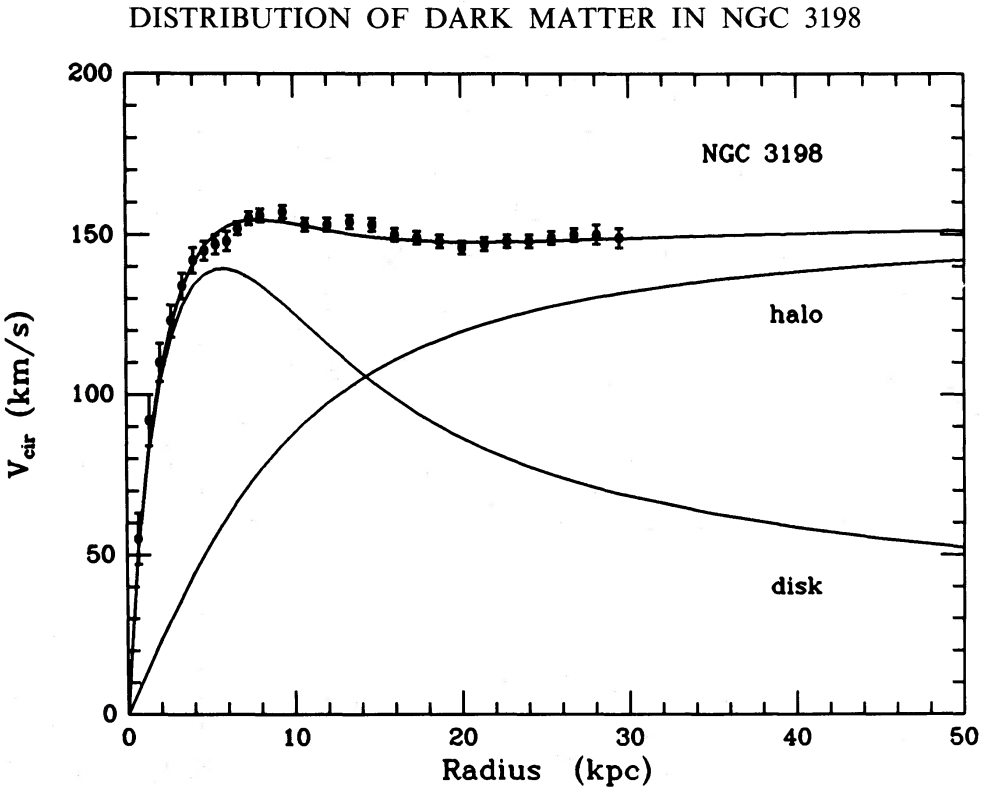
\includegraphics[width=.8\textwidth]{rotation}
\caption{A galaxy rotation curve taken from \citet{vanAlbada1985}. The data points can only be explained by combining the visible `disk' component with an invisible dark matter `halo'.}
\label{co_Fig:rotation}
\end{figure}

More direct evidence for dark matter has been provided by weak lensing mass reconstructions of galaxy cluster collisions, such as those of the Bullet Cluster. The reconstructed matter distribution of this cluster was revealed to extend far beyond its visible limits, and furthermore is inconsistent with a simple modification of gravity at a significance of $8\sigma$ \citep{Clowe2004, Clowe2006}. The observations of the Bullet Cluster also demonstrate the collisionless nature of dark matter \citep{Markevitch2004}.

Further evidence for the existence of dark matter comes from observations of the CMB. Around six times the amount of matter that we observe directly is needed to achieve a good fit to the \lcdm{} model \citep{Planck2018VI}. The CMB will be discussed further in \autoref{co_Sec:CMB}.

Dark matter is required to be `cold', i.e. sufficiently massive as to move non-relativistically, in order to explain the observed level of structure in the present-day Universe \citep{Bond1982, Blumenthal1982, Peebles1982, Blumenthal1984, Davis1985}.

However, despite the relative abundance of observational evidence for dark matter, a direct detection on Earth continues to be elusive. Collider experiments have performed extensive searches over the past decade, and classes of physical models of dark matter that were not long ago believed to be likely have now been largely ruled out \citep{Trevisani2018, Aaboud2018, ATLAS2019}.

\subsubsection{Dark energy}
\label{co_Sec:dark_energy}

Almost all of the remaining energy density in the Universe---around 69.1\% \citep{Planck2018VI}---is believed to be some additional unknown form of energy responsible for the accelerating expansion of the Universe. This additional form of energy is known as dark energy.

\subsubsubsection{Evidence for dark energy}

The main evidence for the existence of dark energy comes from the accelerating expansion of the Universe, which was discovered by precision observations of distant Type Ia supernovae in the late 1990s \citep{Riess1998, Perlmutter1999}. Type Ia supernovae will be discussed further in \autoref{co_Sec:supernovae}. This accelerating expansion cannot be explained under GR without a large additional and previously unknown contribution to the total energy density.

Measurements of CMB anisotropies indicate that the Universe is flat or almost flat \citep{Planck2018VI}. Under the \lcdm{} model, this cannot be explained by matter alone, including dark matter, and therefore requires a large contribution from dark energy. Probes of the large scale structure of the Universe, such as weak lensing, also detect too little matter for flatness \citep[e.g.][]{DES2021}.

\subsubsubsection{Models of dark energy}

\paragraph{Cosmological constant}

The mathematically simplest way to account for an additional energy source in GR and its solutions is with a cosmological constant, $\Lambda$. The cosmological constant was first introduced by Einstein in his original descriptions of GR \citep{Einstein1917} in order to provide a steady state Universe, which was generally assumed to be the case at the time, when his equations otherwise predicted a dynamic Universe. After the Universe was discovered to in fact be expanding, the cosmological constant was assumed to be zero, and Einstein is alleged to have described its initial inclusion as his ``biggest blunder'' \citep{ORaifeartaigh2018}. However, after the accelerating expansion was discovered, the cosmological constant was reinstated and today forms an essential pillar of the \lcdm{} standard model of cosmology.

The cosmological constant gives a dark energy equation of state parameter $w$ of
\begin{equation}
w = -1.
\end{equation}

Physically a cosmological constant corresponds to an intrinsic vacuum energy of space. Such a vacuum energy is predicted by the standard model of particle physics, but is around 120 orders of magnitude too large to explain cosmological observations \citep[e.g.][]{Adler1995}. This is known as the cosmological constant problem, and is one of the major outstanding questions in fundamental physics.

\paragraph{Quintessence}

The term quintessence refers to a proposed new scalar field, many plausible models of which exist (see \citealt{Tsujikawa2013} for a review). Such a field could change over time, such that the dark energy equation of state parameter $w$ is a function of the scale factor $a$,
\begin{equation}
w = w \left( a \right).
\label{co_Eq:quintessence}
\end{equation}

It is common to Taylor expand Equation \eqref{co_Eq:quintessence} to linear order about $a = 1$ to define $\wo$ and $\wa$ as
\begin{equation}
w \left( a \right) = w_0 + w_a \left( 1 - a \right),
\label{co_Eq:w_a_taylor}
\end{equation}
such that
\begin{align}
w_0 &= w \left( a = 1 \right);
\\
w_a &= - \frac{\text{d}w}{\text{d}a} \left( a = 1 \right).
\label{co_Eq:wa}
\end{align}

Observations to date are consistent with the values of
\begin{align}
w_0 &= -1; \\
w_a &= 0
\end{align}
(e.g. \cite{Ribeiro2019}, from a combined analysis of CMB anisotropies, baryon acoustic oscillations, supernovae and cosmic chronometers), which corresponds to a cosmological constant.

\paragraph{Modified gravity}

It is possible to negate the need for dark energy altogether with suitable modifications to gravity, which deviate from GR \citep[e.g.][]{Nojiri2003, Nojiri2011, Nicolis2009, Clifton2012, Nojiri2017}. Alternatively, dark energy could exist alongside a modified theory of gravity. However, all observations to date are consistent with GR, provided that dark energy is included, and some modified gravity models have been ruled out by recent observations of gravitational waves \citep{Blas2016, Vainio2017, Arai2018, Battye2018, Ma2019}. Pulsar timing experiments also place tight constraints on deviations from GR \citep{BeltranJimenez2016, Shao2017, Cai2019, Kramer2021}.

\subsubsection{Other constituents}

The Universe also contains small amounts of `radiation', totalling less than 1\% of the total energy density. This includes neutrinos, and the CMB, which will be described further in \autoref{co_Sec:CMB}.

\subsection{Expansion history}
\label{co_Sec:expansion_history}

The Universe today is dominated by dark energy, but this is a fairly recent development. Prior to this, the Universe is believed to have gone through several epochs in which different components were dominant, each of which will now be described.

\subsubsection{Inflation}

It is believed that the early Universe underwent a short period of rapid expansion, known as inflation \citep{Guth1981, Guth1982, Starobinsky1982,  Linde1982, Linde1983}. The inflationary period is thought to have lasted from $10^{-36}$\,s to $10^{-33}$--$10^{-32}$\,s after the Big Bang, during which the Universe expanded by around 60 $e$-folds (a factor of $10^{26}$) \citep{Planck2018X}. Inflation provides a mechanism to create the seeds for the present-day large-scale structure of the Universe, by vastly magnifying quantum fluctuations in the early Universe. The popularity of the theory is also driven by its ability to solve two significant cosmological problems: the horizon problem and the flatness problem.

The horizon problem is the fact that the CMB is isotropic to within one part in $10^5$, implying that regions far apart on the sky must have been in thermal equilibrium in the early Universe, when---in the absence of inflation---they could have never been in causal contact. Invoking inflation allows seemingly distant parts of the CMB sky to have been in causal contact prior to inflationary expansion.

The flatness problem arises from the observation that the present-day Universe is extremely close to flat \citep{Planck2018VI}. It can be shown from Equations \eqref{co_Eq:friedmann}--\eqref{co_Eq:energy_conservation} that flatness is an unstable equilibrium, in that any perturbation from flatness should grow over time. Therefore, the fact that the Universe is extremely close to flat today implies that any deviation from flatness in the early Universe must have been infinitesimal---of order $10^{-55}$ or smaller \citep{Guth1981}. The lack of an explanation---in the absence of inflation---for this suspiciously convenient value is a type of `fine-tuning' problem. Inflation provides an explanation, because such a rapid expansion of the Universe strongly suppresses any previous cosmic curvature and leaves a Universe sufficiently flat to explain current observations.

Inflation is also able to predict the observed value of the scalar spectral index $n_s$ \citep{Bardeen1983, Planck2018X}. (The scalar spectral index and other parameters of the \lcdm{} model are discussed in \autoref{co_Sec:free_params}.) Physically, inflation can be explained by a new scalar `inflaton' field, many plausible models of which exist \citep[e.g.][for a review]{Bauman2015}. Future CMB polarisation experiments hope to detect direct evidence of the inflaton field, which would confirm the theory of inflation and constrain physical models (see \autoref{co_Sec:CMB}).

\subsubsection{Radiation domination}

The Universe subsequently underwent a period of radiation domination, during which the dominant components were relativistic photons and neutrinos. Radiation is modelled as a gas, exerting a positive pressure in each of three spatial dimensions, giving it an equation of state parameter $w_\text{r}$ of
\begin{equation}
w_\text{r} = \frac{1}{3}.
\end{equation}
Inserting this into Equation \eqref{co_Eq:rho_dependence_on_a} gives the evolution of the radiation density $\rho_\text{r}$ as
\begin{equation}
\rho_\text{r} \propto a^{-4}.
\label{co_Eq:radiation_density_evolution}
\end{equation}
When radiation is dominant, the first Friedmann equation (\autoref{co_Eq:friedmann}) then becomes
\begin{equation}
H^2 \propto a^{-4}.
\end{equation}
Using the definition of the Hubble parameter $H$ in terms of the time derivative of the scale factor (\autoref{co_Eq:hubble_param}), we can obtain a solution for the scale factor as a function of time in the epoch of radiation domination,
\begin{equation}
a \propto t^{1/2}.
\end{equation}

\subsubsection{Matter domination}

The period of radiation domination was followed by a period of matter domination. Matter is pressureless, and therefore its equation of state parameter $w_\text{m}$ is
\begin{equation}
w_\text{m} = 0,
\end{equation}
giving the evolution of the matter density $\rho_\text{m}$ as
\begin{equation}
\rho_\text{m} \propto a^{-3}.
\end{equation}
Comparing this to Equation \eqref{co_Eq:radiation_density_evolution} for radiation explains why matter eventually came to dominate over radiation, since radiation was more heavily diluted by the expansion of the Universe. This effect can be understood in terms of redshift: as the Universe expanded, radiation is redshifted, decreasing its energy by an additional factor $1/a$.

In the epoch of matter domination, the Hubble parameter evolves as
\begin{equation}
H^2 \propto a^{-3},
\end{equation}
which gives the evolution of the scale factor as
\begin{equation}
a \propto t^{2/3}.
\end{equation}
Despite the faster growth of the scale factor during matter domination, it was in this period that structure was most able to form. Structure formation was strongly suppressed in the period of radiation domination by the high density of relativistic particles.

\subsubsection{Dark energy domination}
\label{co_Sec:de_domination}

The Universe is now in a period of dark energy domination. The dark energy equation of state parameter $w$ is either exactly or approximately equal to $-1$, depending on the model (see \autoref{co_Sec:dark_energy}). Inserting a value of $w = -1$, corresponding to a cosmological constant $\Lambda$, into Equation \eqref{co_Eq:rho_dependence_on_a} gives
\begin{equation}
\rho_\Lambda \propto 1,
\end{equation}
i.e. a constant density. This is how dark energy has come to eventually dominate, as the density of matter and radiation is diluted by the expanding Universe. For dark energy domination, Equation \eqref{co_Eq:friedmann} gives that
\begin{equation}
H^2 = \frac{\Lambda c^2}{3},
\end{equation}
which has an exponential solution for the scale factor:
\begin{equation}
a \propto \exp{\left[ \sqrt{\frac{\Lambda}{3}} c t \right]}.
\end{equation}
Under dark energy domination, therefore, the Universe undergoes exponential growth,\linebreak which suppresses structure formation. This means that the growth of structure as a function of redshift $z$ (or equivalently, the scale factor $a$) depends heavily on the nature of dark energy and its potential time evolution. Observational probes of structure growth and the recent expansion history of the Universe are therefore able to potentially place tight constraints on dark energy models via their predictions of $w \left( a \right)$.

\subsection{Density parameters}

It is convenient to define the critical density $\rho_\text{c}$, as the density required for a flat Universe, obtained by setting $K = 0$ and $\Lambda = 0$ in Equation \eqref{co_Eq:friedmann}:
\begin{equation}
\rho_\text{c} = \frac{3 H^2}{8 \pi G}.
\end{equation}
For each component $X$ of the Universe, we may then define the density parameter $\Omega_\text{x}$,
\begin{equation}
\Omega_\text{x} = \frac{\rho_\text{x}}{\rho_\text{c}}.
\end{equation}
We may include the curvature contribution to the Friedmann equation in this form too by defining it as a density $\rho_K$,
\begin{equation}
\rho_K = -\frac{3 K c^2}{8 \pi G a^2},
\end{equation}
giving the curvature density parameter $\Omega_K$,
\begin{equation}
\Omega_K = \frac{\rho_K}{\rho_\text{c}}
= -\frac{K c^2}{a^2 H^2}.
\end{equation}
Including a general dark energy contribution, the Friedmann equation (\autoref{co_Eq:friedmann}) may then be written in form which makes explicit the way in which the different components evolve over time:
\begin{equation}
\frac{H^2}{H_0^2} =
\frac{\Omega_\text{r}}{a^4} +
\frac{\Omega_\text{m}}{a^3} +
\frac{\Omega_K}{a^2} +
\frac{\Omega_\text{DE}}{a^{3 \left( 1 + w \right)}}.
\label{co_Eq:freidmann_as_omegas}
\end{equation}
If dark energy is a cosmological constant, then the last term in Equation \eqref{co_Eq:freidmann_as_omegas} becomes simply $\Omega_\Lambda$, with
\begin{equation}
\Omega_\Lambda = \frac{\Lambda c^2}{3 H^2}.
\end{equation}

\subsection{Free parameters}
\label{co_Sec:free_params}

The minimal \lcdm{} model has six free parameters. There is not a single unique parameterisation, but a typical choice is the following \citep[e.g.][]{DiValentino2015}:

\begin{itemize}
\item The Hubble parameter $H_0$, which may alternatively be described using the dimensionless Hubble parameter $h$,
\begin{equation}
h = \frac{H_0}{100\,\text{km}\,\text{s}^{-1}\,\text{Mpc}^{-1}}.
\label{co_Eq:h_definition}
\end{equation}
\item $\omb h^2$, where $\omb$ is the energy density of baryons as a fraction of the critical density.
\item $\omc h^2$, where $\omc$ is the dark matter energy density as a fraction of the critical density.
\item The amplitude of primordial scalar perturbations $A_s$.
\item The scalar spectral index $n_s$, describing the scale dependence of primordial perturbations.
\item The optical depth to reionisation $\tau$: a physical description of the redshift of the epoch of reionisation, which was a period in the evolution of the Universe when the first stars and other luminous sources were formed, and were able to ionise hydrogen in the intergalactic medium.
\end{itemize}

Other parameters may be derived from these six, and vice versa. The parameters that are constrained by a particular experiment will depend on the cosmological probe in question. Two derived parameters that are of interest in this thesis are:
\begin{itemize}
\item $\omm$, the total matter density, given by
\begin{equation}
\omm = \omc + \omb.
\end{equation}
\item $\sie$, the amplitude of present-day matter fluctuations on scales of $8\,h^{-1}\,\text{Mpc}$. This may be constrained directly by probes of large scale structure, but can also be predicted by the \lcdm{} model given the free parameters listed above.
\end{itemize}

The \lcdm{} model may be extended by adding additional parameters. One extension is of particular interest in this thesis, which is the extension to time-varying dark energy via a dark energy equation of state parameter that depends on the scale factor as $w \left( a \right)$. As introduced in Equations \eqref{co_Eq:w_a_taylor}--\eqref{co_Eq:wa}, this may be Taylor expanded to linear order to define $w_0$ and $w_a$, which are the two cosmological parameters of greatest interest to this thesis. The extension to \lcdm{} to include $w_0$ and $w_a$ is often called \wcdm{}.

Current constraints on the ten parameters listed above are given in \autoref{co_Tbl:params}. These are taken from \citet{Planck2018VI}, where they are derived from CMB temperature, polarisation and lensing, combined with baryon acoustic oscillations and, for the dark energy parameters $w_0$ and $w_a$, Type Ia supernovae. Each of these probes is described in \autoref{co_Sec:obs_probes}.

\begin{table}
\caption{Current constraints on the ten cosmological parameters described in \autoref{co_Sec:free_params}. Taken from \citet{Planck2018VI} Tables 2 and 6, where they are derived from CMB temperature, polarisation and lensing, combined with baryon acoustic oscillations and, for $w_0$ and $w_a$, Type Ia supernovae.}
\label{co_Tbl:params}
\vspace{.5em} % for some reason I couldn't find a way to automate this
\centering
\bgroup
\def\arraystretch{1.5}
\begin{tabular}{ll}
% \hline
Parameter & Best-fit value $\pm$ 68\% limits \\
\hline
$H_0 \left[ \text{km}\,\text{s}^{-1}\,\text{Mpc}^{-1} \right]$
& $67.66 \pm 0.42$ \\
$\omb h^2$ & $0.02242 \pm 0.00014$ \\
$\omc h^2$ & $0.11933 \pm 0.00091$ \\
$10^9 A_s$ & $2.105 \pm 0.030$  \\
$n_s$ & $0.9665 \pm 0.0038$ \\
$\tau$ & $0.0561 \pm 0.0071$ \\
\hline
$\omm$ & $0.3111 \pm 0.0056$ \\
$\sie$ & $0.8102 \pm 0.0060$ \\
\hline
$\wo$ & $-0.957 \pm 0.080$ \\
$\wa$ & $-0.29\substack{+0.32 \\ -0.26}$
\end{tabular}
\egroup
\end{table}

\section{Outstanding questions}
\label{co_Sec:open_questions}

The previous section has described in some detail the current best understanding of the nature of the Universe. However, many questions remain outstanding. Below is a brief summary of a selection of key open questions in cosmology.

\begin{itemize}
\item \textbf{Nature of the constituents.} As described in \autoref{co_Sec:constituents}, around 95\% of the energy density of the Universe consists of dark energy and dark matter. However, the physical nature of both of these components remains unknown, along with an explanation for why the cosmological constant does not correspond to the vacuum energy predicted by the standard model of particle physics.
\item \textbf{Modified gravity.} Is GR correct, or is a modified theory of gravity required?
\item \textbf{Inflation.} What is the physical nature of the mechanism responsible for inflation?
\item \textbf{Tensions in measured parameters.} It is common for different experiments to infer values of cosmological parameters that are not in perfect agreement. However, two particular discrepancies have arisen between experiments measuring the late-time Universe and the early Universe. The most significant of these is the tension in the Hubble parameter $H_0$, between local measurements of Type Ia supernovae calibrated by Cepheid variable stars using the distance ladder method (which will be described in \autoref{co_Sec:supernovae}), and values inferred from CMB observations conditioned on the \lcdm{} model. This tension between early and late time measurements is illustrated in \autoref{co_Fig:h0_tension}. This figure is taken from \citet{DiValentino2021Hubble}, since which the tension has been claimed to have reached the $5 \sigma$ significance level \citep{Riess2021b}. The second tension of interest is in the parameter $S_8$, defined as\footnote{The power of $0.5$ in Equation \eqref{co_Eqn:s8} is sometimes varied slightly depending on the best fit to the data, such as to $0.48$ in \citet{Rhodes2001}.}
\begin{equation}
S_8 = \sigma_8 \left[ \frac{\omm}{0.3} \right]^{0.5},
\label{co_Eqn:s8}
\end{equation}
between local measurements using weak lensing compared to those inferred from CMB observations. This tension is currently claimed to stand at the 2--3$\sigma$ level based on one recent weak lensing analysis from the Kilo-Degree Survey \citep{Heymans2021}, although better agreement with the CMB is found by the Dark Energy Survey \citep{DES2021}. (Both of these current weak lensing surveys will be described in \autoref{co_Sec:observational_history}.) While the $S_8$ tension may just be a statistical fluke, or the result of undiagnosed systematic errors, the $H_0$ tension has persisted and strengthened despite being repeatedly examined with increasing care \citep[e.g.][]{Riess2018b, Riess2018c, Riess2018a, Riess2020, Riess2021a, Riess2021b, Burns2018, Yuan2019, Reid2019, Macaulay2019, Soltis2021, Anand2021, Romaniello2021}, and a resolution may require new physics \citep{DiValentino2021Hubble}.
\end{itemize}

\begin{figure}
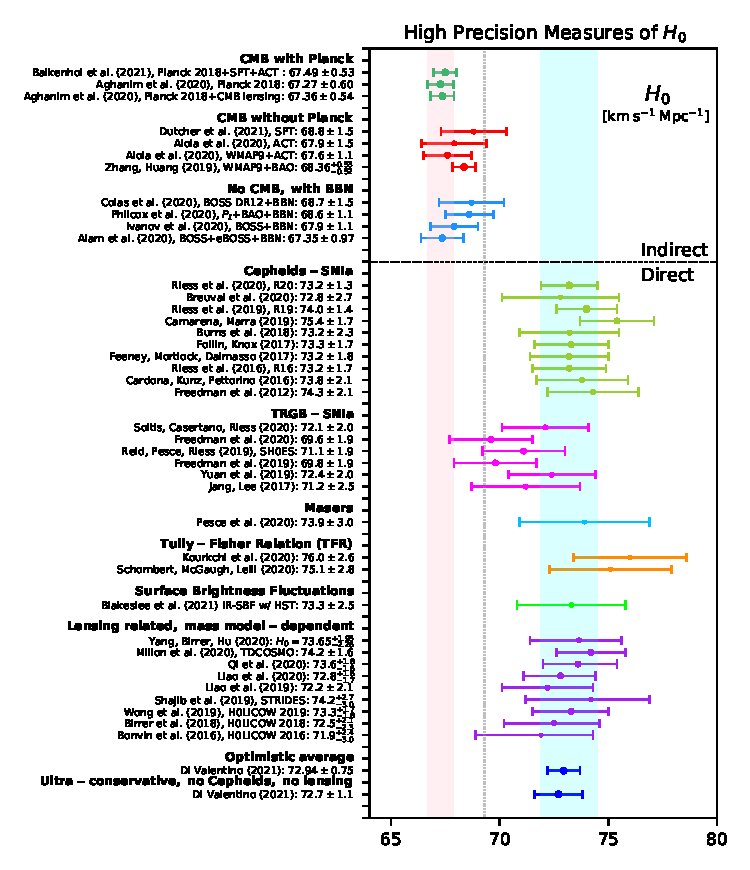
\includegraphics[width=\textwidth]{h0_tension}
\caption{Tension in measurements of the Hubble parameter $H_0$ between early (indirect) and late time (direct) observations. Figure taken from \citet{DiValentino2021Hubble}. Error bars are 68\% credible intervals. The blue band corresponds to the result from \citet{Riess2020} and the pink to those from \citet{Planck2018VI}.}
\label{co_Fig:h0_tension}
\end{figure}

\section{Observational probes}
\label{co_Sec:obs_probes}

There are a number of observational methods by which our current best understanding of the Universe, as described in \autoref{co_Sec:std_model}, has been developed, and using which we hope to answer some of the remaining outstanding questions such as those summarised in \autoref{co_Sec:open_questions}. A selection of these methods are described in this section.

\subsection{Cosmic microwave background}
\label{co_Sec:CMB}

\begin{figure}
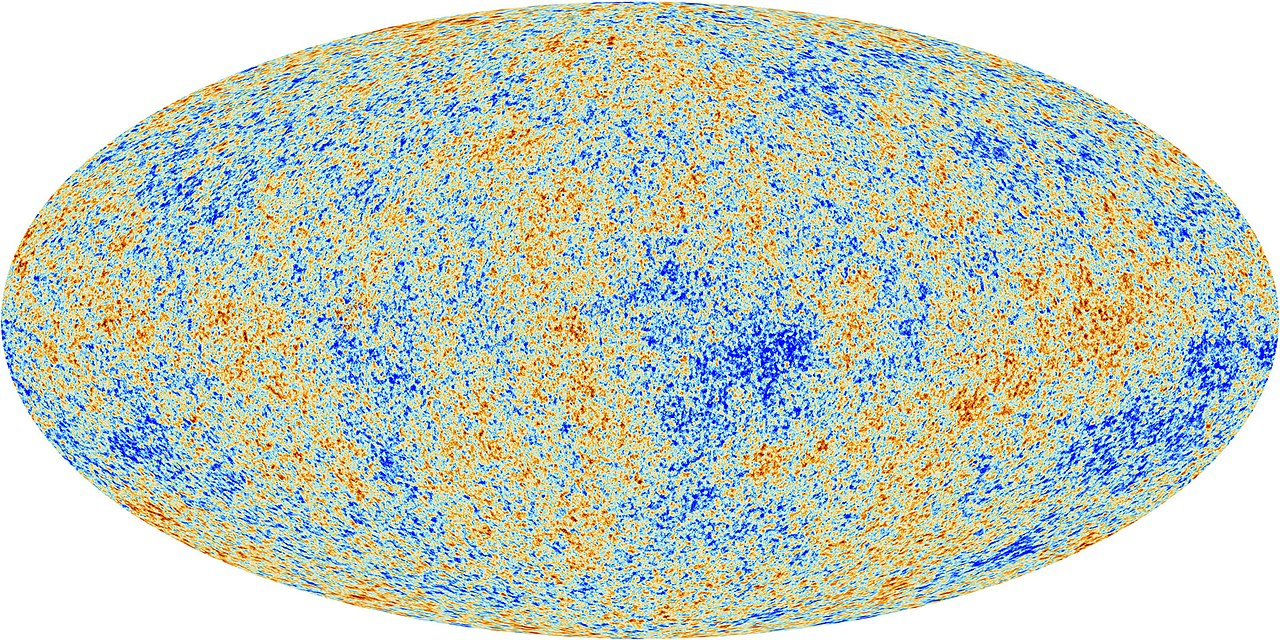
\includegraphics[width=\textwidth]{planck_t}
\caption{Map of CMB temperature anisotropies measured by the \Planck{} satellite \citep{Planck2018I}. Red colours are warmer than average and blue colours cooler, both by up to $300\,\mu\text{K}$.}
\label{co_Fig:planck_t}
\end{figure}

Observations of the cosmic microwave background (CMB) have perhaps offered more insight into the nature of the Universe than any other method. The CMB consists of photons from the early Universe that have been redshifted over time and now reside in the microwave regime, corresponding to a temperature of around 2.7\,K.

The origin of the CMB can be traced back to the first $\sim$\,380\,000 years after the Big Bang, during which the Universe was sufficiently hot that it was impossible for atoms to form without being ionised, and high-energy photons existed in thermal equilibrium with protons and electrons. As the Universe expanded, it cooled, and eventually the photons had insufficient energy to ionise atoms, and the first hydrogen atoms were born. This period, called recombination, occurred at a redshift of $z \sim 1100$.

The CMB contains small anisotropies in both its temperature and polarisation, of order one part in $10^5$ and $10^6$ respectively, which are understood to be the precursor to the large-scale structure in the present-day Universe. (Baryon acoustic oscillations, discussed in \autoref{co_Sec:BAO} below, provide strong evidence for this link between the early and late time Universe.) The scale dependence of these anisotropies, captured by the power spectrum (see \autoref{chap:est_like}), are predicted by the \lcdm{} model and depend closely on its free parameters. As a result, observations of the CMB are able to constrain many cosmological parameters, such as the amount of baryonic matter, dark matter, dark energy and curvature in the Universe, as well as its age and properties of primordial perturbations.

The CMB was proposed and discovered---initially by accident---in the mid-20th century \citep{Gamow1948a, Gamow1948b, Alpher1948a, Alpher1948b, Doroshkevich1964, Penzias1965, Dicke1965}. A series of satellite missions in the late 20th and early 21st centuries made increasingly precise observations, free from interference from terrestrial radio sources. The first was the NASA Cosmic Background Explorer (COBE) mission, which operated from 1989 to 1993 and confirmed that the CMB radiation has an almost perfect blackbody spectrum, consistent with theoretical predictions \citep{Fixsen1996}. It was also able to measure the intrinsic anisotropies for the first time \citep{Bennett1996}. The anisotropies were measured to much higher precision with the subsequent NASA Wilkinson Microwave Anisotropy Probe (WMAP) mission, which operated from 2001 to 2010 and was able to resolve smaller scale features in the CMB temperature power spectrum. Finally, the ESA \Planck{} mission, which operated from 2009 to 2013, achieved higher resolution still, as well as measuring anisotropies in the polarisation of the CMB. The map of CMB temperature anisotropies from the \Planck{} mission is shown in \autoref{co_Fig:planck_t}. The final cosmological analysis of \Planck{} data in \citet{Planck2018VI} stands as the current pinnacle of precision cosmology, achieving sub-percent precision in many cosmological parameters.

Current and future CMB experiments such as the South Pole Telescope \citep{Carlstrom2011}, the Atacama Cosmology Telescope \citep{Swetz2011}, the POLARBEAR experiment \citep{Kermish2012}, the Simons Observatory \citep{so2019}, CMB-S4 \citep{Abazajian2016} and LiteBIRD \citep{Hazumi2019} have science goals including the detection of direct evidence of inflation via the measurement of primordial $B$-mode polarisation \citep{Kamionkowski2016} and the measurement of spectral distortions, which probe the thermal history of the Universe \citep{Chluba2019, Chluba2021}.

\subsection{Gravitational lensing}
\label{co_Sec:gravitational_lensing}

Gravitational lensing is the name given to the distortion of light by gravity. It was predicted by GR \citep{Einstein1916, Einstein1936}, in which gravity is modelled as a consequence of the distortion of spacetime by an uneven distribution of mass,
% which has the effect of bending the path of light as well as massive objects.
which has the effect of not only bending the paths of massive objects but also of light.
The prediction was confirmed soon afterwards, with measurements of the deflection of the images of stars by the gravity of the Sun during a solar eclipse \citep{Dyson1917, Dyson1920}.

\begin{figure}
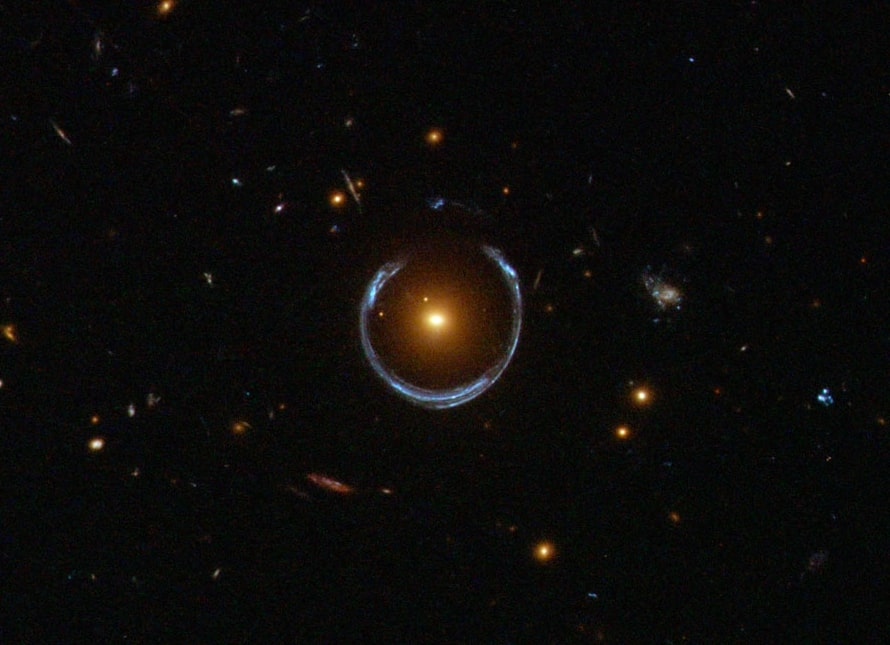
\includegraphics[width=\textwidth]{strong_lens}
\caption{A strong lensing event captured by the Hubble Space Telescope, in which a distant blue galaxy is lensed by a foreground red galaxy. Image credit: ESA/Hubble \& NASA.}
\label{co_Fig:strong_lens}
\end{figure}

Occasionally the alignment of a source and lens object is such that strong lensing occurs, in which the image of the source is distorted so strongly that the lensing effect is obvious without the need for any statistical analysis. An example is shown in \autoref{co_Fig:strong_lens}, in which the image of a distant blue galaxy has been strongly lensed by a foreground red galaxy. Analysis of strong lensing events like this can help to constrain models of dark matter and gravity, since the precise distortion of the source image depends sensitively on these factors \citep[e.g.][]{Vegetti2014, Li2016, Hezaveh2016, Gilman2020, Andrade2022}. Strong lensing observations have also been used to constrain the Hubble parameter $H_0$, because strong gravitational fields not only distort images but also the time taken for light to pass through the field \citep[e.g.][]{Bonvin2017}.

Strong lensing is rare, but essentially every line of sight on the sky is lensed weakly to some degree. This means that observations of distant galaxies are able to trace the large scale structure of the Universe through weak lensing. Weak gravitational lensing is the main observational probe of cosmology considered in this thesis, and is described in more detail in \autoref{co_Sec:weak_lensing}.

\subsection{Type Ia supernovae}
\label{co_Sec:supernovae}

Type Ia supernovae are the end-life stage of binary star systems in which one or both stars is a white dwarf. Accretion onto the white dwarf from its companion eventually takes it beyond a certain threshold mass, which triggers runaway nuclear fusion leading to a supernova explosion.

The usefulness of Type Ia supernovae to cosmology lies in the fact that this fixed critical mass---around 1.44 solar masses---leads to all Type Ia supernovae exploding at the same peak brightness. Such an object of known brightness is known as a standard candle, and allows the calculation of the distance to the object by comparison with the apparent brightness from Earth. Although Type Ia supernovae are thought to all have the same intrinsic peak brightness, this brightness is not itself predicted by theory. This necessitates the calibration of the brightness using observations of supernovae whose distance is known by some other means. A common method involves observations of Cepheid variables in the same galaxies as the supernovae. Cepheid variables are pulsating stars, whose pulsation period is related to their brightness, such that the same method can be used to determine their distance by measuring their pulsation period. The relationship between period and brightness has to itself be calibrated, using parallax measurements of nearby Cepheids. This method of repeated calibration to obtain reliable distance measurements is known as the cosmic distance ladder.

Observations of distant Type Ia supernovae were used to detect cosmic acceleration \citep{Riess1998, Perlmutter1999}, and are still regularly used for determining the Hubble constant $H_0$ \citep{Dhawan2018, Burns2018, Macaulay2019, Taubenberger2019, Khetan2021, Riess2021a, Riess2021b}.

\subsection{Baryon acoustic oscillations}
\label{co_Sec:BAO}

Baryon acoustic oscillations are a particular scale dependence in the large-scale matter distribution in the present-day Universe. They arise from acoustic waves in the early Universe prior to recombination, which were formed from the counteracting forces of gravity and radiation pressure surrounding overdense regions of the primordial plasma. In this period, baryons and photons were coupled, but following recombination the photons free-streamed away to form the CMB, relieving the radiation pressure and leaving the baryons essentially frozen in shells of a particular size. This size is given by the sound horizon at the time of recombination, which can be predicted by theory and has been confirmed to high precision by CMB observations \citep{Planck2018I}. These shells evolved gravitationally to form a distinct signal in the late-time matter distribution in the Universe. Measurements of the baryon acoustic oscillation signal in large-scale structure provide a clear link between scales in the early and late Universe, while measurements of the signal as a function of redshift directly probe the expansion history of the Universe. This defined scale is known as a standard ruler, by analogy with standard candles such as Type Ia supernovae described in \autoref{co_Sec:supernovae} above.

Baryon acoustic oscillations have been detected in the past two decades by galaxy surveys including the Sloan Digital Sky Survey (SDSS; \citealt{Eisenstein2005, Percival2010}), the 2dF Galaxy Redshift Survey (2dFGRS; \citealt{Cole2005}), the 6dF Galaxy Survey (6dFGS; \citealt{Beutler2011}), the WiggleZ Dark Energy Survey \citep{Blake2011, Kazin2014} and the SDSS (extended) Baryon Oscillation Spectroscopic Survey (BOSS/eBOSS; \citealt{Anderson2012, Anderson2014, Delubac2015, deSainteAgathe2019, Blomqvist2019}).

\subsection{Redshift-space distortions}

Redshift-space distortions are distortions of galaxy positions in redshift space relative to their positions in real space, due to additional contributions to their redshift beyond the dominant Hubble expansion. These can be due to orbital Doppler shifts, or general relativistic gravitational redshift. Observations of redshift-space distortions can be used to constrain models of cosmological structure formation \citep{Percival2009, Macaulay2013, Howlett2015} as well as testing GR and constraining theories of modified gravity \citep{Beutler2014, Percival2011, Raccanelli2013}.

\subsection{Gravitational waves}

Gravitational waves are travelling distortions of spacetime emanating from accelerating masses. They are predicted by GR \citep{Einstein1916, Einstein1918} but were only recently directly detected for the first time, by the Laser Interferometer Gravitational-Wave Observatory (LIGO) and the Virgo Interferometer \citep{Abramovici1992, Accadia2012, Abbott2016}. Gravitational wave detections are useful as a test of GR, and have already imposed significant constraints on modified gravity models \citep{Blas2016, Vainio2017, Arai2018, Battye2018, Ma2019}. Gravitational waves resulting from black hole or neutron star mergers may be used to constrain cosmic expansion if accompanied by an electromagnetic detection, since the gravitational wave signal can be used to deduce distance while the electromagnetic signal provides redshift, thus directly constraining the Hubble constant $H_0$ via Equation \eqref{co_Eqn:hubble_law} \citep{Abbott2017}. Future gravitational wave observatories such as the Kamioka Gravitational Wave Detector (KAGRA; \citealt{Akutsu2019}) and the space-based Laser Interferometer Space Antenna (LISA; \citealt{Amaro-Seoane2017}) may be able to probe inflation by detecting a gravitational wave background from the early Universe \citep{Bartolo2016, Caprini2019, Maggiore2020, Kawamura2021}.

\subsection{Hydrogen 21\texorpdfstring{\,}{ }cm line}

The Hydrogen 21\,cm line is an emission line caused by a spin-flip in neutral hydrogen, between two states with an energy difference of around $5.9\,\upmu\text{eV}$, leading to an emission wavelength of around $21.1$\,cm.
Since the distribution of neutral hydrogen follows the large-scale structure of the Universe, the 21\,cm line can be used a probe of the large-scale structure. In a low-redshift context, this can have similar uses to other probes of large-scale structure such as galaxy surveys; for example, to constrain models of dark energy and modified gravity \citep{Hall2013, Bull2015}. However, much attention is focused on high-redshift observations of the 21\,cm line, since it is the only known way to probe the `dark ages' between recombination and reionisation. This is an important period of structure growth in the Universe, during which the first stars and galaxies were formed.
% Due to the current lack of observational data from this period, these processes are relatively poorly understood.
High-redshift 21\,cm observations will probe this early growth of structure, which should tightly constrain the properties of dark matter as well as potentially revealing signals from the early Universe \citep{Furlanetto2006, Pritchard2012}.

Measurements of the 21\,cm line are challenging due to the faintness of the signal and interference from other radio sources, both terrestrial and astrophysical. However, it has been estimated that future radio observatories such as the Square Kilometre Array (SKA; see \autoref{co_Sec:future_wl_surveys}) will be sufficiently sensitive to measure the power spectrum of the 21\,cm line at the epoch of reionisation, provided foreground sources are sufficiently well understood \citep{Pober2014}.

\section{Weak gravitational lensing}
\label{co_Sec:weak_lensing}

Weak gravitational lensing is the main observational probe of cosmology considered in this thesis. This section gives a qualitative description of weak lensing as a cosmological probe, while some of the more mathematical aspects are introduced in \autoref{chap:est_like}.

As discussed in \autoref{co_Sec:gravitational_lensing}, light paths may be distorted by passing through gravitational fields. This means that in principle, the light observed in any direction on the sky has been subtly distorted by the mass distribution between the source and the observer. This offers particular value when applied to distant galaxies: the shape of each galaxy is subtly distorted by everything along the line of sight from the galaxy to the observer on Earth. For cosmologically distant galaxies with redshifts up to $z \sim$ 1--2, there is potentially a large amount of matter along the line of sight to contribute to this distortion.

In principle, if the undistorted shape of a galaxy were known, it could be compared with the observed shape to infer the projected mass distribution to the galaxy. In practice, the intrinsic shape of a specific individual galaxy is unknown, but progress may be made with a statistical treatment of a large number of galaxies. If, to first order, we assume that galaxies are oriented randomly with no preferential alignment (which is not quite true in practice; see the section on intrinsic alignments in \autoref{co_Sec:wl_challenges}), then we can look out for a preferred alignment of a large number of galaxies in a particular part of the sky to uncover the projected mass distribution in that region. Repeating this process over the whole sky can probe the entire projected large-scale structure of the Universe, out to the limiting redshift of the survey. Weak gravitational lensing by the large-scale structure of the Universe is known as cosmic shear.

The scientific value of a weak lensing analysis can be increased further using the technique of tomography: splitting source galaxies into bins depending on their redshift. This gains two additional sources of information: first, redshift corresponds to distance, which introduces three-dimensional information about the large-scale structure. Second, redshift corresponds to time, which introduces information amount the late-time evolution of structure. This is why weak lensing is such a promising probe of dark energy: as discussed in \autoref{co_Sec:de_domination}, the evolution of structure in the recent Universe depends heavily on the nature of dark energy, and specifically its equation of state parameter $w \left( a \right)$. Weak lensing also probes everything to do with matter, and therefore is a valuable tool to constrain the properties of dark matter. Its unique advantage relative to other probes of large scale structure such as galaxy clustering is that it only depends on mass distributions and the lensing theory predicted by GR, and not on additional factors such as galaxy bias.

\subsection{Combination with galaxy clustering}

It is common to combine weak lensing and galaxy clustering analyses. Galaxy clustering is the statistical analysis of the positions of galaxies on the sky, often as a function of redshift, which---similar to weak lensing---traces the large-scale structure of the late-time Universe.
% Since weak lensing requires measuring the shapes of large numbers of galaxies, it is relatively little additional work to also record their positions in order to include galaxy clustering in the analysis.
Since weak lensing necessarily requires measuring the shapes and positions of large numbers of galaxies, galaxy clustering may also be included in the analysis for relatively little additional work.

The advantage of combining weak lensing and galaxy clustering data lies in their respective challenges and sources of systematic error. Dominant sources of systematic uncertainty in weak lensing analyses such as shape estimation and intrinsic alignments, both of which are discussed in \autoref{co_Sec:wl_challenges} below, do not apply to galaxy clustering, while model uncertainties in the relationship between the positions of galaxies relative to their local dark matter distribution are irrelevant to weak lensing. Combining the two types of data can therefore reduce the importance of these sources of systematic error, while increasing the statistical power of the analysis \citep[e.g.][]{Abbott2018}.

Combined weak lensing and galaxy clustering analyses typically also include the cross-correlation of galaxy positions and shapes, known as galaxy-galaxy lensing. As well as probing the evolution of large-scale structure, galaxy-galaxy lensing offers valuable insight into galaxy evolution \citep[e.g.][]{Zacharegkas2022}.

\subsection{Challenges in weak lensing}
\label{co_Sec:wl_challenges}

Weak lensing analyses are fraught with many challenges and sources of systematic error. Some of the most significant of these are now discussed.

\paragraph{Intrinsic alignments}

It is not necessarily safe to assume that all the source galaxies in a weak lensing analysis are randomly oriented prior to any lensing. Tidal forces during galaxy formation can lead to galaxies being aligned to their local large-scale dark matter structure. This leads to a preferential alignment among physically nearby galaxies, which could be misinterpreted as a lensing signal. Additionally, a foreground galaxy could be intrinsically aligned to its local large-scale structure, which lenses a background galaxy, also causing a spurious signal---this time an anti-correlation. Both effects have been measured in real data \citep{Brown2002, Hirata2004, Joachimi2011, Mandelbaum2011, Singh2015}.

The effect of intrinsic alignments may be mitigated in broadly one of two ways: either by downweighting certain nearby galaxy pairs \citep{Heymans2003, Heymans2004, Joachimi2008ia} or by modelling the effect directly \citep{Bridle2007, Schneider2010, Blazek2015, Blazek2019, Fortuna2021, Samuroff2021, Harnois-Deraps2022}. Since the processes that cause intrinsic alignments are not well understood, such models typically involve several free parameters which must be marginalised over to incorporate the model uncertainty into cosmological parameter constraints \citep[e.g.][]{Joachimi2010, Troxel2015, Amon2021}.

\paragraph{Redshift determination}

In an ideal scenario, the redshift of each galaxy in a weak lensing analysis would be determined using spectroscopy: measuring the full spectrum of the galaxy, identifying key features with known rest-frame wavelengths and comparing to their observed wavelengths to determine the redshift with high confidence. However, the galaxies in a real weak analysis are too numerous and too faint to determine spectroscopic redshifts for all but a small fraction of the sample. Instead, photometric redshifts are used: galaxy flux is measured in a few different bands, and these measurements are used to estimate the redshift of the galaxy. This is a necessary but highly uncertain method, which has the potential to introduce serious biases into cosmological results if not properly treated \citep{Sun2009, Hearin2010}. The optimal treatment of photometric redshifts and the reduction of potential induced biases are significant areas of active research within weak lensing \citep{DIsanto2018, Graham2018, Bilicki2018, Pasquet2019, Amaro2019, Leistedt2019, Boucaud2020, Wright2020, Schmidt2020, Schuldt2021, Henghes2021, Cordero2021, Lima2022, Rau2022}. In practice, much uncertainty remains, and it is therefore still necessary to marginalise over many nuisance parameters describing photometric redshift uncertainty in a real analysis \citep[e.g.][]{Heymans2021, DES2021}.

\paragraph{Shape determination}

There are several challenges to determining galaxy shapes sufficiently accurately and precisely to detect a cosmic shear signal, which is an effect of order per cent. One such challenge is the point spread function (PSF) of the telescope, which must be known to a very high precision in order to avoid misinterpreting its effect as a shear signal \citep{Kuijken1999, Jarvis2004, Rhodes2007, Rowe2010, Chang2012, Lu2017, Eriksen2018, Zhang2022}. Another is overlapping galaxies on the sky, known as blending, which is an inevitable consequence of the large numbers of galaxies included in weak lensing analyses. Mistakenly identifying two overlapping galaxies as a single galaxy can cause biases, but so too can naively removing galaxies identified as overlapping, since this would create a selection bias against higher density regions \citep{Dawson2016, Hoekstra2021, Gaztanaga2021, Sanchez2021, Melchior2021,  Nourbakhsh2021}. A third class of challenges in shape determination is detector systematics, such as charge transfer inefficiency \citep{Rhodes2010} and the brighter-fatter effect \citep{Walter2015, Gilbertson2017, Coulton2018, Rowlands2018, Freudenburg2020}.

\paragraph{Modelling of non-linear scales}

Regardless of how accurately and precisely observational measurements can be made, final cosmological results are still limited by the ability to model all physical effects reliably. A particular challenge in this regard lies in the modelling of small physical scales. The growth of structure on such scales and the effect of astrophysical feedback processes are poorly understood and difficult to model. There is disagreement between different models, and between model predictions and simulations \citep{Casarini2011, Schneider2016, Giblin2019, Bose2019, Bose2020}. This is a highly active area of ongoing study, and is likely to limit the scales at which future weak lensing data can be analysed reliably \citep{Huterer2005, Jing2006, vanDaalen2011, Semboloni2011, Semboloni2013, Zentner2013, Mohammed2014, Eifler2015, MacCrann2017, Copeland2018, Huang2019, Huang2021, Martinelli2021}. Choosing such scale cuts carefully can isolate well-understood scales while extracting maximal cosmological information \citep{Kitching2011, Taylor2018, Deshpande2020, Taylor2021a, Taylor2021b}.

\paragraph{Cosmic variance}

Cosmic variance describes the principle that the value of any cosmological observable measured from Earth is just one sample from the distribution of this observable over the entire Universe, which of course extends far beyond the most distant galaxies in a weak lensing survey \citep{Kamionkowski1997, Wiltshire2007, Driver2010, Moster2011}. In practice, what this means is that even given perfect knowledge of both theory and experiment, the value of a cosmological observable cannot be predicted exactly; it is instead given by a probability distribution. In some ideal cases, we may know the form of this distribution, but more generally it is necessary to make approximations. Inverting the argument above implies that, even with perfect knowledge of an experiment and no uncertainty of any kind on the observed data, we will necessarily still have non-zero error bars on the inferred cosmological parameters \citep[e.g.][]{Martel1998, Taylor2010}.

A consequence of cosmic variance is that it demands a statistical treatment of all observables in cosmology.
%Statistical modelling is a challenge, and is the main focus of this thesis.
As the precision achieved by cosmological experiments increases, so too must the level of understanding of the statistical properties of all aspects of the data. Upcoming weak lensing experiments such as \Euclid{} (see \autoref{co_Sec:Euclid}) will offer an unprecedented level of precision, due to the extremely large numbers of observed galaxies. This level of precision demands an equally unprecedented level of refinement in statistical modelling, which is the main focus of this thesis. The mathematical concepts involved in this statistical modelling of cosmology, and specifically weak lensing, will be introduced in \autoref{chap:est_like}.

\subsection{Observational history of weak lensing}
\label{co_Sec:observational_history}

The first successful observations of weak lensing by large scale structure were made in 2000 by four separate teams. \citet{VanWaerbeke2000} used the Canada France Hawaii Telescope (CFHT) to survey 191\,000 galaxies over an area of $6300\,\text{arcmin}^2$, detecting cosmic shear on scales from 0.5 to 3.5\,arcmin. \citet{Wittman2000} claimed a detection on scales up to 30\,arcmin, from 145\,000 galaxies imaged using the Big Throughput Camera \citep{Wittman1998} on the 4\,m Blanco telescope at the Cerro Tololo Inter-American Observatory. Detections were also made by \citet{Bacon2000} using the 4.2\,m William Herschel Telescope \citep{Boksenberg1985} over a total area of $1792\,\text{arcmin}^2$, and by \citet{Kaiser2000} using the CFHT with around 120\,000 galaxies over an area of $5400\,\text{arcmin}^2$.

More surveys followed in the early 2000s. The first space-based weak lensing survey was carried out using the Hubble Space Telescope (HST), surveying 4000 galaxies in the $168\,\text{arcmin}^2$ HST survey strip using the Wide Field Planetary Camera 2 \citep{Griffiths1990}, to place constraints on $S_8$ (\autoref{co_Eqn:s8}) with a one-third error bar at 68\% posterior probability \citep{Rhodes2001}. This was improved upon with the Red-Sequence Cluster Survey \citep{Gladders2001}, which covered $53\,\text{deg}^2$ using both the CFHT and Cerro Tololo Inter-American Observatory 4\,m telescope and included 1\,773\,543 galaxies, to place constraints on $S_8$ with a 27\% error at 95\% posterior probability \citep{Hoekstra2002a, Hoekstra2002b}. The COMBO-17 survey covered $1.25\,\text{deg}^2$ using the La Silla 2.2\,m telescope in Chile \citep{Wolf2001}, including 83\,514 galaxies, and further improved constraints on $S_8$ to 12.5\% at 68\% posterior probability \citep{Brown2003}. Further surveys followed: $2.1\,\text{deg}^2$ using the Suprime-Cam \citep{Miyazaki2002} at the Subaru Telescope \citep{Hamana2003}; the Cerro Tololo Inter-American Observatory Survey of 2 million galaxies covering $75\,\text{deg}^2$ \citep{Jarvis2003}; the VIRMOS-Descart survey using the CFHT \citep{VanWaerbeke2005}; and the HST GEMS Survey using the Advanced Camera for Surveys, including 71\,233 galaxies over $795\,\text{arcmin}^2$ in the \textit{Chandra} Deep Field South with an extremely high galaxy number density of $60\,/\,\text{arcmin}^2$, compared to a more typical value of $\sim 30\,/\,\text{arcmin}^2$ \citep{Heymans2005}.

The CFHT Lensing Survey (CFHTLenS; \citealt{Heymans2012}) was the first to have sufficient numbers of galaxies across a range of redshifts to place constraints on the expansion of the Universe and its acceleration, via the dimensionless Hubble parameter $h$ and the dark energy equation of state parameter $w$.
CFHTLenS was an optical imaging survey based on $154\,\text{deg}^2$ of data taken with the CFHT between 2003 and 2009 as part of the CFHT Legacy Survey. It included around 6 million galaxies with shape and photometric redshift estimates, across a redshift range from $z = 0.5$ to $1.3$. The survey produced a number of constraints on cosmology \citep{Kilbinger2013, Benjamin2013, Heymans2013, VanWaerbeke2013, Kitching2014, Fu2014} including values of $h = 0.78 \pm 0.12$ and $w_0 = -1.10 \pm 0.15$ (68\% credible interval) when combined with WMAP data. There have also been several reanalyses combining CFHTLenS data with other external data \citep[e.g.][]{More2015, Blake2016, Joudaki2017}.

Three large weak lensing surveys are currently ongoing. This generation are known as Stage III surveys, based on the definitions set out in the Report of the Dark Energy Task Force \citep{Albrecht2006} regarding their ability to constrain dark energy. These are the Hyper Suprime-Cam Subaru Strategic Program Survey, the Kilo-Degree Survey, and the Dark Energy Survey.

The Hyper Suprime-Cam Subaru Strategic Program (HSC SSP; \citealt{Aihara2018}) is a $1400\,\text{deg}^2$ optical imaging survey with the HSC \citep{Miyazaki2012} on the 8.2\,m Subaru Telescope in Hawaii. To date an area of $670\,\text{deg}^2$ has been observed and released publicly \citep{Aihara2021}, but the only cosmological analysis so far is of the Year 1 data, comprising 9 million galaxies over $137\,\text{deg}^2$ with a redshift range of $z =$ 0.3--1.5. This obtained a constraint of $S_8 = 0.780\substack{+0.030 \\ -0.033}$ at 68\% posterior probability \citep{Hikage2019}. No meaningful constraints on dark energy were possible with the first year data alone, but should be possible with the $\sim$ 90 million galaxies expected to be observed in the full survey.

The Kilo-Degree Survey (KiDS; \citealt{DeJong2013}) is a $1350\,\text{deg}^2$ optical imaging survey, carried out with the OmegaCAM \citep{Kuijken2011} on the VLT Survey Telescope at the Paranal Observatory in Chile. To date, an area of $1006\,\text{deg}^2$ has been observed and released publicly (KiDS-1000; \citealt{Kuijken2019}). The main cosmological analysis from this data set included 21 million galaxies over a redshift range of $z = $0.1--1.2 \citep{Giblin2021}, and obtained a constraint of $S_8 = 0.766\substack{+0.020\\-0.014}$. As mentioned in \autoref{co_Sec:open_questions}, this value is discrepant with that from \Planck{} CMB data \citep{Planck2018VI} at $\sim$2--3$\sigma$ \citep{Heymans2021}.

\begin{figure}
\centering
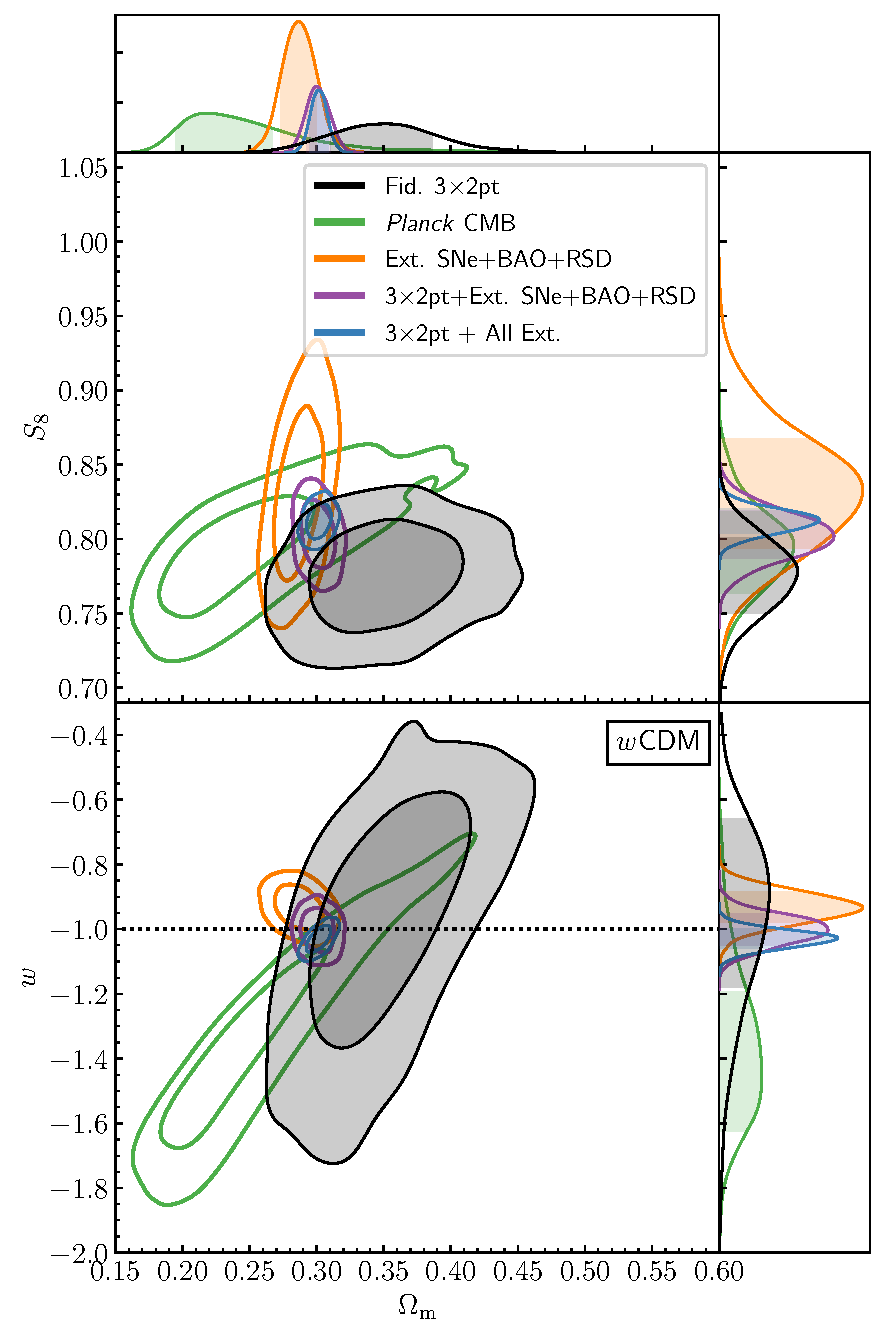
\includegraphics[width=.8\textwidth]{des_y3}
\caption{Cosmological constraints from the Dark Energy Survey Year 3 analysis \citep{DES2021}. Each panel shows the 68\% and 95\% credible regions of joint constraints on two parameters marginalised over all other parameters. The grey contours show the constraints from DES data alone, while the blue constraints include \Planck{} CMB data, baryon acoustic oscillations, redshift-space distortions and Type Ia supernovae. Other colours show other combinations of data.}
\label{co_Fig:des_y3}
\end{figure}

The Dark Energy Survey (DES; \citealt{DES2005}) is a six-year optical imaging survey on the Dark Energy Camera \citep{Flaugher2015} at the Blanco 4\,m telescope at the Cerro Tololo Inter-American Observatory in Chile. 300 million galaxies were observed between 2013 and 2019, but to date only 100 million have been included in published cosmological analyses \citep{DES2021}. The survey covers $5000\,\text{deg}^2$ and includes galaxies out to redshift $z = 2$. The Year 3 cosmological analysis reports results of $S_8 = 0.775\substack{+0.026\\-0.024}$ and $w = -0.98\substack{+0.32\\-0.20}$, from DES data alone. Combined with \Planck{} CMB data, plus baryon acoustic oscillations, redshift-space distortions and Type Ia supernovae, they obtain $S_8 = 0.812 \pm 0.08$; $w = -1.031\substack{+0.030\\-0.027}$; $h = 0.687\substack{+0.006\\-0.007}$. Some parameter constraints from the Year 3 analysis are shown in \autoref{co_Fig:des_y3}. To obtain these results, such methodological advances were necessary that the collaboration published 29 methods papers for the Year 3 analysis alone \citep[and references therein]{DES2021}. The future Year 6 analysis will require still further refinement to reliably extract the maximum information from all 300 million sources.

\subsection{\Euclid{} satellite}
\label{co_Sec:Euclid}

\Euclid{} \citep{Laureijs2011} is an upcoming European Space Agency (ESA) satellite mission. It was born from a combination of two satellite proposals to ESA: the Dark Universe Explorer (DUNE; \citealt{Refregier2009}), a weak lensing mission, and the Spectroscopic All Sky Cosmic Explorer (SPACE; \citealt{Cimatti2009}), a spectroscopic galaxy clustering mission to measure baryon acoustic oscillation and redshift-space distortions. As such, \Euclid{} is equipped with two complementary instruments: an optical imager---VIS---and a near-infrared spectrometer \& photometer---NISP. \Euclid{} is scheduled to be launched in early 2023 from the ESA spaceport in French Guiana, into an orbit around the $L_2$ Sun--Earth Lagrange point.

Over a nominal lifetime of six years, \Euclid{} will survey $15\,000\,\text{deg}^2$ of the extragalactic sky (the Euclid Wide Survey; \citealt{Scaramella2021}) out to a magnitude of 26.2 with VIS and 24.5 with NISP.
It is expected to survey around 10 billion galaxies in total, with around 1.5 billion having sufficiently precise shape and photometric redshift estimates for use in the weak lensing analysis. These source galaxies will have redshifts out to $z \sim 2$, with the majority having $z \sim 1$. Around 23 million galaxies will have precise spectroscopic redshift estimates made using NISP. There will also be three deep fields, together covering $40\,\text{deg}^2$ to form the Euclid Deep Survey, which will reach about two magnitudes deeper than the wide survey.

\begin{figure}
\centering
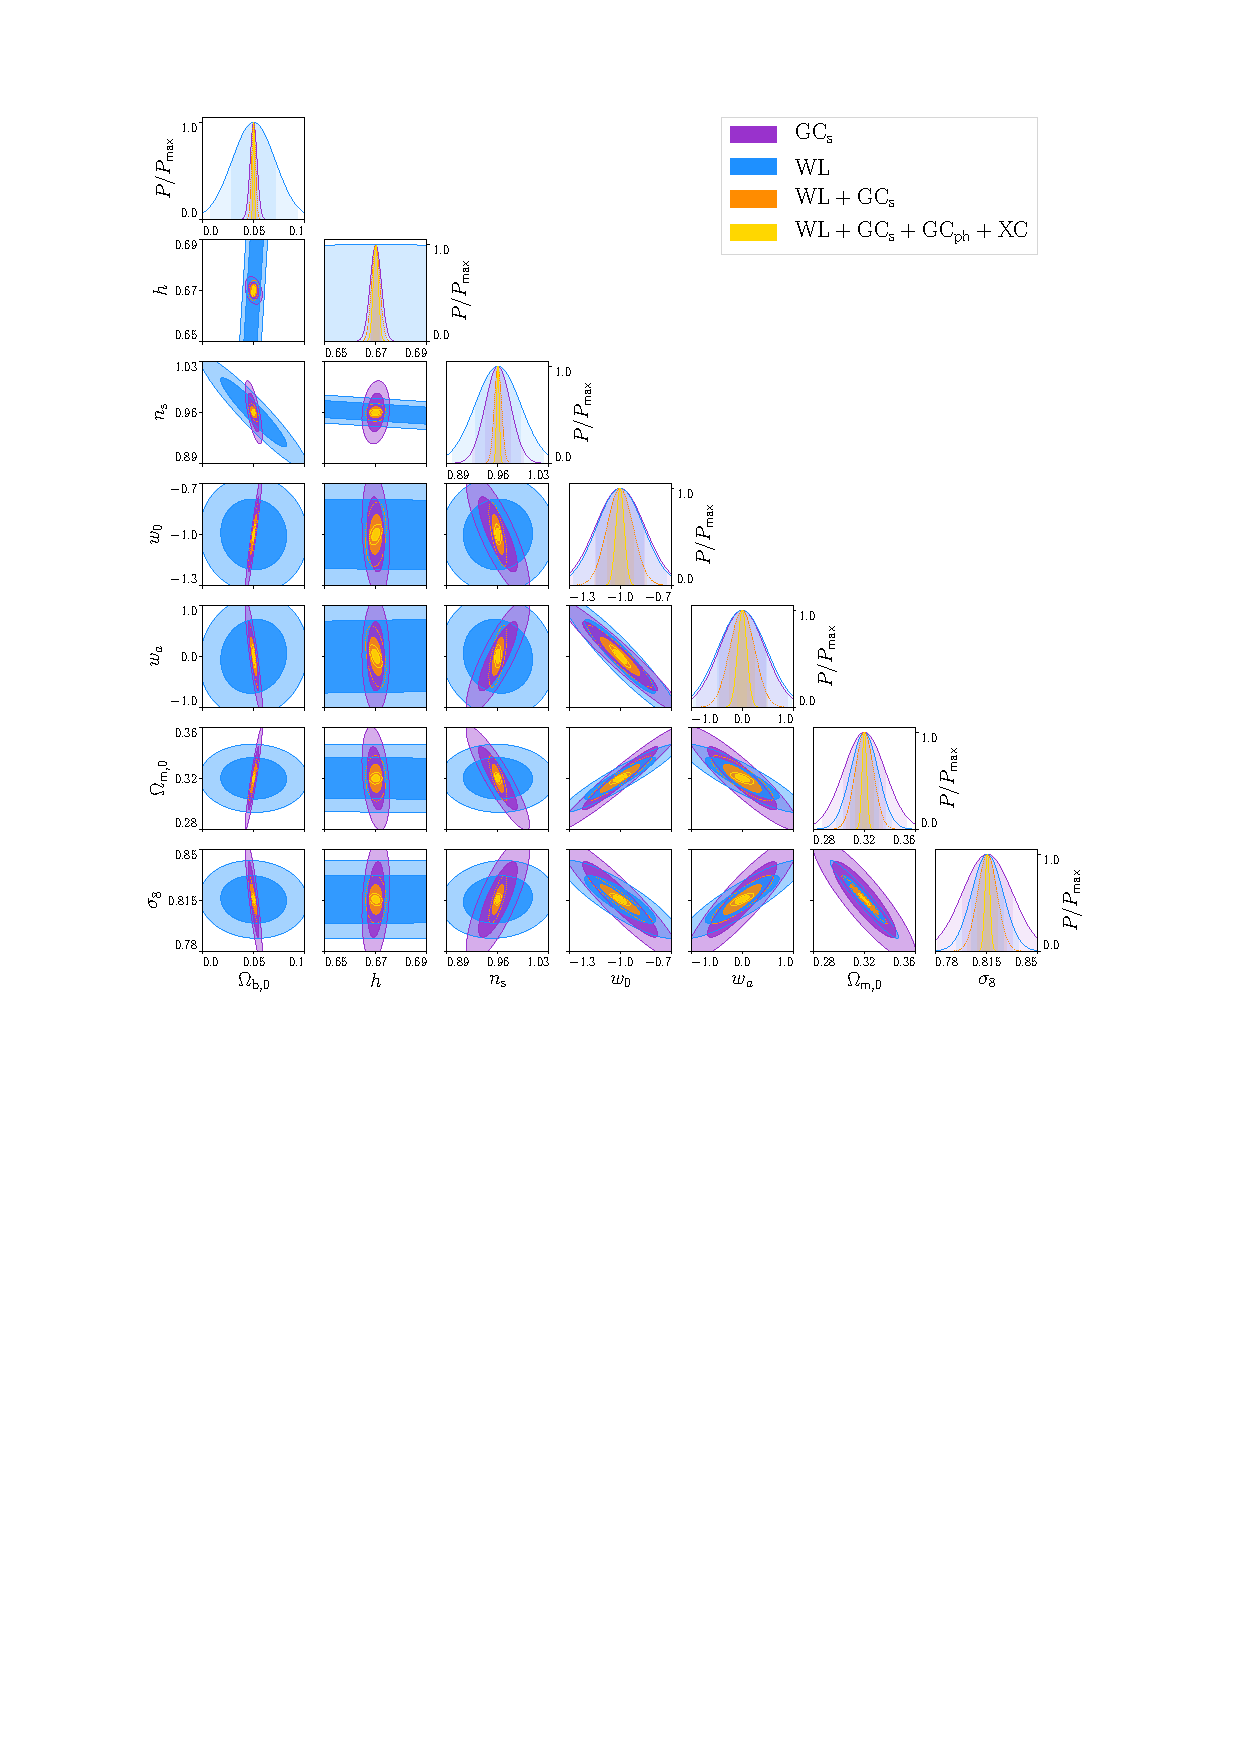
\includegraphics[width=\textwidth]{euclid_forecast}
\caption{Forecasted constraints for \wcdm{} parameters from future \Euclid{} data, combining spectroscopic galaxy clustering (GC${}_\text{s}$), weak lensing (WL), photometric galaxy clustering (GC${}_\text{ph}$) and cross-correlations (XC). Taken from \citet{Blanchard2020}.}
\label{co_Fig:euclid_forecast}
\end{figure}

The \Euclid{} cosmological analysis will use weak lensing and spectroscopic galaxy clustering, plus photometric galaxy clustering and its cross-correlation with weak lensing \citep{Blanchard2020}. Using these probes, it will determine the late-time evolution of the large-scale matter distribution in the Universe, and measure baryon acoustic oscillations and redshift-space distortions. The main scientific goal is to constrain dark energy, constraints on which are expected to improve by over an order of magnitude relative to current Stage III surveys \citep{Harrison2016}. \Euclid{} will also be able to tightly constrain other parameters of the \wcdm{} model, as shown in \autoref{co_Fig:euclid_forecast}, as well as theories of modified gravity.

The preparation and initial data analysis is conducted by the Euclid Consortium, which currently contains over 1400 people in 17 countries globally. After the initial analysis, data will be released to the public, where it is expected to have a big impact on legacy science. Potential non-cosmology uses include studies of galactic physics, and stellar physics within the Milky Way.

\subsection{Other future surveys}
\label{co_Sec:future_wl_surveys}

There are at least three other Stage IV weak lensing surveys planned alongside \Euclid{}. The first is the Vera C. Rubin Observatory Legacy Survey of Space and Time (LSST; formerly the Large Synoptic Survey Telescope; \citealt{Ivezic2019}). Rubin is a brand new ground-based observatory in Chile, which will conduct an optical imaging survey of around $18\,000\,\text{deg}^2$ of the southern sky. It has similar goals to \Euclid{} of constraining dark energy and structure growth, with some complementary characteristics; for example, \Euclid{} will have higher angular resolution, but Rubin will be able to detect fainter objects. This means that there is great potential from combining data from the two experiments \citep{Rhodes2017, Guy2022}. The survey is scheduled to last for ten years, starting in 2023.

\Euclid{} is expected to be joined at the $L_2$ point by the Nancy Grace Roman Space Telescope (formerly the Wide-Field Infrared Survey Telescope; \citealt{Spergel2015}), a NASA satellite currently scheduled to launch by May 2027. It will carry two instruments: a wide-field optical and near-infrared camera used primarily for a galaxy survey, alongside a coronograph for directly imaging exoplanets. Like \Euclid{} and Rubin, the main cosmological aim of Roman is to constrain dark energy. To do so, it will survey around $2000\,\text{deg}^2$ of the extragalactic sky over a period of around 24 months. It will be sensitive to magnitudes up to 28.5, so should be able to detect fainter galaxies than \Euclid{}, with a superior angular resolution due to its larger telescope, to compensate for the smaller survey area.

Finally, the Square Kilometre Array (SKA; \citealt{SKA2020}) is expected to be able to perform weak lensing analyses using radio observations. The SKA is a radio array currently under construction in Australia and South Africa, expected to begin observations in some capacity in the next decade. Use of the SKA for weak lensing has several key advantages compared to optical surveys such as \Euclid{} \citep{Harrison2016}: it will probe a broader redshift distribution, potentially out to $z \sim 6$; there is less PSF contamination for radio observations; intrinsic alignments may be able to be directly measured using radio polarisation \citep{Brown2011, Whittaker2015}; and it has the ability to access more of the sky, since the Galaxy is effectively transparent to radio interferometers. However, the greatest benefits are gained by cross-correlating radio and optical data, since this not only unlocks additional constraining power but also significantly reduces the impact of systematic errors, which are largely different for radio and optical surveys \citep{Camera2017}.


% % Uncomment to build alone without subfiles:
% \emergencystretch=.5em % to avoid overfull hboxes
% \printbibliography[heading=bibintoc]
% \end{document}
